
\chapter{Pushing the limit of \pangenome construction methods}
\label{sec:pushing}
In this first chapter I present and discuss two projects in which I have pushed the current limit of \pangenome constructing methods to provide useful insight of their features, of their relative advantages and of the improved capabilities compared to current genomic approaches.\\ In the first one I have analyzed the current state of the art methods available at the moment and stress-tested them by also generating what was, to the best of my knowledge, the largest human \pangenome produced at the time. \\ The second one is the generation of a yeast \pangenome reference for the species \emph{Lodderomyces elongisporus}, with some of the tools used in the aforementioned work, to demonstrate how pan-genomes are a superior representation to investigate cross-chromosomal rearrangements compared to the linear reference used by commonly used genomic tools. In order to best capture this large rearrangement between three chromosomes, I had to modify and customize one of the most used variation graph pangenome construction pipeline and compared to other two graphs. Here I present the challenges faced, discuss which data structure to use to achieve biological correctness, genome variation resolution, scalability or downstram application usability and show how a \pangenome enables improved analysis of inter-chromosome rearrangements.

\section{Motivation}
The paper that follows this section originates from a discussion early in my PhD journey on which were the best tools suited for large cohort \pangenome construction, specifically for large 
Eukaryote genomes, like primates. As pointed out in the introduction, there is no one-fits-all solution and most of the tools, at the time of the analysis, were freshly released or distributed under development. It was therefore important for the community of developers and users of such new tools and models to understand the limitations and the potential of the new pan-genomic methods.\\
In order to perform a thorough assessment of the best available methods, we tried to mimic the conditions that they could face in the near future. We therefore decided to test on the largest collection of high quality human data as it is paramount to understand how pangenomes can be used and adapted to be the platform of future large genomic studies.\\
As introduced in section~\ref{sec:background_pangenomics}, there are multiple ways of representing a group of genomes to be analyzed or used jointly. One that took traction in the last few years has been graphs. Graphs can represent the sequences as labels of nodes, relationship between them (adjacency or overlap) as edges and infer difference in the genomes as different set of nodes in them.\\
We specifically focused our attention on the most used graph models: variation graphs and De Bruijn Graphs. In variation graph edges represent adjacencies, i.e the genome is spelled by a walk on nodes connected by an edge. In De Bruijn Graphs they represent overlaps, i.e. the suffix of a node is the prefix of the next node connected to it: this implies that edges can exists between nodes that are not adjacent in the genome. As discussed in the next sessions, this distinction implies several differences in how these graphs can be used for downstream analysis. \\ 
In this article, we surveyed the the methods and tools that build such graphs, then tested them on different dataset sizes and permutations, and finally analyzed the resulting representation's features. The outcome is a small guide on which are the best applications for each of these tools and an analysis of how they represent variations in genomes. \\
%The work we performed was intended for publication, but, to the best of my knowledge, the manuscript has never been put in production.

\author
{
	Francesco Andreace
	\and
	Pierre Lechat
	\and
	Yoann Dufresne
	\and
	Rayan Chikhi
}
\title{Comparing methods for constructing and representing human pangenome graphs}

\metadata
{
	Published in \emph{Genome Biology},
	November~2023,
	volume~24,
	issue~1,
	article number 274.
	\doi{10.1186/s13059-023-03098-2}.
}
\maketitle
\label{pap:first}

\begin{abstract}
	\textbf{Background:} As a single reference genome cannot possibly represent all the variation present across human individuals, pangenome graphs have been introduced to incorporate population diversity within a wide range of genomic analyses. Several data structures have been proposed for representing collections of genomes as pangenomes, in particular graphs. \\
	\noindent \textbf{Results:} In this work we collect all publicly available high-quality human haplotypes and construct the largest human pangenome graphs to date, incorporating 52 individuals in addition to two synthetic references (CHM13 and GRCh38). We build variation graphs and de Bruijn graphs of this collection using five of the state-of-the-art tools: \bifrost, \mdbg, \minigraph, \mcactus and \pggb. We examine differences in the way each of these tools represents variations between input sequences, both in terms of overall graph structure and representation of specific genetic loci. \\
	\noindent \textbf{Conclusion:} This work sheds light on key differences between pangenome graph representations, informing end-users on how to select the most appropriate graph type for their application.
\end{abstract}

\startcontents[chapters]
\printcontents[chapters]{}{1}{\section*{\contentsname}}

\section{Introduction}
In recent years, the majority of studies on human genetics have been conducted on the basis of comparing new samples against a single, standard reference sequence. This reference sequence is a linear succession of nucleotides that acts as a blueprint of the human genome. It is routinely used to align raw sequencing data to it in order to find variations between genomes, e.g. single-nucleotide polymorphisms (SNPs), insertions or deletions (indels). It also is the backbone of the UCSC Genome Browser~\cite{ucsc} which enables inspection of genomic and epigenomic features. Despite updates that have improved the quality of the human reference sequence in the last two decades, its linear form severely limits the ability to capture population genetic diversity. For instance the locations of frequently observed structural variations cannot be easily integrated into a linear reference. To see this, consider the difficulty of designing a suitable coordinate system in the presence of (possibly nested) structural variants. Having a single genome as reference sequence also introduces an observational bias towards the chosen alleles that were integrated into that sequence, negatively impacting many primary analyses such as reads mapping, variant calling, genotyping and haplotype phasing. As a result our ability to precisely characterize structural variants, SNPs and small indels is limited \cite{vg,computational_pangenomics,giraffe}. The GRCh38 human reference genome is estimated to miss up to 10\% of our species genetic information \mbox{\cite{human-pangenomics-era}}.

Improvements in sequencing data quality and length, as well as  genome assembly methods, are providing a fast expanding collection of haplotype-resolved human genome assemblies. If adequately combined together, these high-quality individual genomes may offer an powerful alternative to the linear reference. There now is an active line of research on pangenomes, i.e. data structures that represent a collection of genomic sequences to be analyzed jointly or to form a reference \cite{computational_pangenomics,hpp}. 

Pangenome-based approaches have been shown to improve biological analyses. Pangenomes are at the basis of bioinformatics tools that perform high-quality short read mapping \mbox{\cite{giraffe}}, genotyping of SNPs, indels and SVs \mbox{\cite{pangenie}}, RNA-seq mapping \mbox{\cite{hdpr}}; de novo variant calling \mbox{\cite{vg}}; to store, compress and retrieve high quality genomes \mbox{\cite{gbz}}; to condensate all the information from a high number of genomes to then visualize specific regions or perform ad-hoc analysis, particularly on complex loci, SVs and tandem repeats \mbox{\cite{hdpr}}.
These results pave the way for new applications, e.g. genome-wide association studies, where more precise identification of variants can improve the scope of genetic studies in aging, human diseases, and cancer~\cite{computational_pangenomics, hpp}.

Several pangenomic data structures have been proposed: multiple sequence alignments, de Bruijn graphs, cyclic and acyclic variation graphs, and haplotype-centric models that use the Burrows-Wheeler transform ~\cite{computational_pangenomics}. Each of these approaches aim to represent a collection of genomic sequences in an efficient way, to store, visualize, and retrieve differences of interest between the considered genomes. 
Graph-based pangenome data structures, such as the de Bruijn graph and the variation graph, appear so far to be the most advanced in their ability to handle large amounts of input data. They are capable of representing tens to hundreds of human haplotypes simultaneously. Variations graphs use a sequence graph and a list of paths to store input haplotypes, while de Bruijn graphs store all haplotype \kmers annotated by their haplotype(s) of origin. 
Scaling pangenome graph data structures to store hundreds of genomes is a challenge that requires significant computational resources and engineering efforts. Many software tools have been created, here we briefly describe major ones.
Pantools~\cite{pantools} and Bifrost~\cite{bifrost} are two methods that have been developed to generate pangenomes for analysis on large collections of genomes, mostly for applications in phylogenetics and bacterial genomics. The PanGenome Graph Builder (\pggb)~\cite{pggb}, \mcactus and \twopaco~\cite{twopaco} are methods for building general-purpose pangenome graphs. \minigraph~\cite{minigraph} builds a particular type of pangenome graph by aligning sequences in an iterative way to a reference template. Minimizer-space de Bruijn graphs (\mdbg)~\cite{mdbg} are variants of de Bruijn graphs that can efficiently represent very large collections of bacterial pangenomes (e.g. 600,000 bacteria).  \mbox{\vg}~\mbox{\cite{vg}} builds variation graphs from a reference sequence and a variant calling file (vcf) that contains a list of variations from it.
Many human pangenomes have been generated, e.g. using Pantools~\cite{pantools} (7 genomes),  \minigraph~\cite{minigraph} (94 haplotypes), \mcactus~\cite{cactus,mcactus} and \pggb~\cite{hdpr} (94 single chromosomes), and \twopaco~\cite{twopaco} (100 simulated genomes). Lastly, a draft version of a human reference pangenome constructed using \pggb\ and the \mcactus pipeline has appeared in a very recent article from the Human Pangenome Reference Consortium~\cite{hdpr}.
These pangenomes are still limited by some factors: at the present moment, the number of high-quality haplotype assemblies is still low, even if it is expected to grow in the future; the vcf files containing variation are limited in term of bias, type of variation or number of samples; the population representation, even if opened up in recent years to more ethnicities, is still affected by sampling bias.

\section{Results}
In this article we provide a comprehensive view of whole-genome human pangenomics through the lens of five methods that each implement a different graph data structure: \mbox{\bifrost}, \mbox{\mdbg}, \mbox{\minigraph}, \mbox{\mcactus} and \mbox{\pggb}. We examine several features of pangenome graphs, in particular their scalability and how they represent genetic diversity. To this end we collected all publicly available high-quality human haplotypes and attempted to construct pangenomes of various complexity with each selected tool.
Although \mbox{\vg} has been widely used at the basis of relevant pangenome-based discoveries, for example on fast and accurate short read mapping \mbox{\cite{giraffe}}, we decided to not consider it in our analysis for two main reasons: the bias introduced by the reference sequence that is used as the backbone of the graph (and associated to the vcf) together with the limited capacity of this method to integrate structural variations from many genomes. We believe both aspects are drivers of the use of pangenome graphs.
\begin{figure}[htp]
	\centering
	\includegraphics[width=0.95\textwidth]{figures/paperI/scheme.jpg}
	\caption[The complete human pangenome construction scheme and visualization.]{\textbf{The complete pangenome construction scheme and visualization.} \textbf{A}, The overall workflow, using 5 different tools on 3 different datasets; \textbf{B}, complete 104 haplotypes variation graph built by \minigraph; \textbf{C}, focus on part of HLA (MHC) region in chromosome 6 from panel B; \textbf{D}, focus on DRB1-5 locus of HLA from panel C; \textbf{E}, complete 10 haplotypes variation graph built with \pggb; \textbf{F}, 10 haplotypes variation graph built with \mcactus; \textbf{G}, 104 haplotypes pangenome \mdbg; \textbf{H}, 10 haplotypes \bifrost \dbg. All graphs except those produced by \minigraph have been simplified using gfatools and rendered using \bandage. VG is for variation graph.}
	\label{fig:figure1}
\end{figure}


\subsection*{\textbf{Scalability and characteristics of pangenome graph construction tools \label{sec:results}}}
\label{sec:scalablility}
We ran the above five tools on three datasets consisting of 2, 10, and 104 human haplotypes respectively (Table~\mbox{\ref{tab:datasets}}). We compared the computational performance of construction algorithms as well as characteristics of the produced pangenome graphs.
The goal is to assess the ability of each method to scale to data available in the near future, i.e. thousands or even millions of human genomes~\cite{human-pangenomics-era}. \\

The performance of each tool is evaluated in terms of running 

, peak memory, disk space required by the output data structure (graph and annotations). We also compared the number of nodes, edges and connected components as indicators of the complexity of the graph. Results are displayed in Table \ref{tab:computational_metrics}. 

In terms of running time, \mdbg is two orders of magnitude faster than other tools on all considered datasets, taking around two minutes on the H2 dataset and half an hour on H104.
\bifrost is the second fastest on H104 (18 hours), and \minigraph is the second fastest on H2 (8 minutes). \mcactus takes one order of magnitude more time than \minigraph. We could not obtain graphs for \pggb and \mcactus on H104 as for the first execution did not finish after 2 weeks and the second returns an error. 

In terms of memory usage, \mdbg consistently uses less than half the memory of other tools (31 GB on H104), followed by \minigraph (61 GB on H104). On H2 all tools used between 8 and 66 GB of memory.

All tools used reasonable disk space to store the resulting graph, $\leq 12$ GB for H10 and $\leq 38$ GB for H104. Although \mcactus and \pggb retain all variations and are the only two tools able to reconstruct the input haplotypes directly from the graph, they are the second and third most efficient in term of disk space (for \mcactus, 3.6 GB on H2 and 7 GB on H10). 
While \bifrost and \minigraph perform all computation in memory, \pggb, \mcactus, and \mdbg store intermediate files on disk, taking comparable space to the input size (up to 3x for \mcactus).  \\

\subsection*{\textbf{Different tools yield different pangenome graphs topologies}}
Graph metrics such as the number of nodes, edges and connected components provide useful insights on the level of detail of the represented variations and on the complexity and accessibility of the information inside the pangenome.

The number of graph nodes varies between 17,000 and 11 millions for the H2 dataset across all tools. In all cases, the number of nodes is at least 3 orders of magnitude smaller than the number of bases in the haplotypes, indicating that pangenome graphs are effective at compressing linear parts of the haplotypes.
Tools which discard variations (\minigraph and \mdbg) yield in the order of $10^4$--$10^5$ nodes across all datasets, while tools which retain all variation (\bifrost, \mcactus and \pggb) yield in the order of $10^6$--$10^7$ nodes. In all cases going from the H10 dataset to the H104 dataset increases the number of nodes by 5x, indicating that graph complexity grows sublinearly with the number of added haplotypes.

The number of connected components varies between 2 and 1402 across all methods and datasets, and the number of large components (i.e. those with more than 1\% of total base pairs) varies between 1 and 30. 
If chromosomes were separated perfectly, pangenome graphs should contain exactly 24 connected components (one per nuclear chromosome, excluding mitochondria). \minigraph produces 24 large connected components as the number of chromosomes in the reference CHM13 v2.0 (25 including mitochondria).
\bifrost and \mcactus yield graphs with less than 25 connected components  while \mdbg and \pggb have more than 25.
In the \bifrost \dbg, the vast majority of sequences ($>$99.99\%) are in a single giant component, as chromosomes are joined because they share common \kmers. In \mdbg such joining does not occur on dataset H2, which has 24 large enough components (each containing $>$ 1\% of bases), possibly due to the absence of long and similar enough regions between chromosomes. 
\minigraph does not map any mitochondrial sequence from the input haplotypes to the reference, while they do get included into \mcactus graphs.

Even if it is common practice to analyze pangenomes chromosome by chromosome~\cite{hdpr,mcactus}, in this analysis we purposely used entire genomes as input instead. This was done for two reasons: i) to highlight the scalability of the tools, and ii) because separating chromosomes prevents the identification of inter-chromosomal inversions, translocations, and transposable elements, even if most of the generated inter-chromosomal events are probably alignment artifacts.
The effects of this choice can be seen in the \pggb and the \mcactus H10 variation graphs of Figure~\ref{fig:figure1}. In the \pggb graph 19 chromosomes are linked into a single giant component, while chromosomes 17, 18, 20, X, and Y are in other large components. This giant component consists of 25 M nodes that contain  83\% of the total basepairs. The remaining 859 components represent only 4.7\% of the total bases due to small sequences in the input haplotypes. 
In the \mcactus graph all chromosomes are linked into a single giant component except chromosome 18 that is in a separate component, and the sexual chromosomes (X and Y) that are connected together into another component.

\begin{table}
	\centering
	\caption[Computational metrics comparison between pangenome building tools.]{Time, memory, final disk space, nodes, edges, total connected components and connected components with more than 1\% of base pairs comparison of \bifrost, \mdbg, \pggb, \minigraph and \mcactus for different number of haplotypes in input. \mcactus times include the \minigraph graph construction step. \pggb was not able to complete its execution on the largest dataset in more than 2 weeks thus it is not considered. \mcactus failed to compute the 104 HAP dataset.}
	\resizebox{\textwidth}{!}{
		\begin{tabular}{|c c c c c c c|} 
			\hline
			Haplotypes & Metric &    \bifrost & \pggb & \minigraph & \mcactus & \mdbg\\
			\hline \hline
			\multirow{7}{*}{2}  &  time  (hh:mm:ss)  & 1:21:25  & 15:45:30 & 00:08:33 & 3:11:59 & 00:02:38\\
			\cline{2-7}
			& memory (GB)  & 53 & 24 & 38 & 66 & 8 \\
			\cline{2-7}
			& disk space (GB) &  4.8 & 4.3 & 2.9 & 3.6 & 4.4\\
			\cline{2-7}
			& nodes   & 9,482 k   &  8,492 k & 34 k & 10,851 k & 17 k\\
			\cline{2-7}
			& edges   & 13,108 k  & 11,503 k &  48 k & 14,702 k & 23 k\\
			\cline{2-7}
			& conn comp  & 2 & 1402 & 25 & 4 & 174\\
			\cline{2-7}
			& conn comp $>$ 1\% bp & 1 & 30 & 24 & 4 & 24\\
			
			\hline\hline
			\multirow{7}{*}{10}  & time (hh:mm:ss) &   2:27:29  &  117:08:09 & 2:03:29  & 15:57:05 & 00:05:46\\
			\cline{2-7}
			& memory (GB) & 102  & 71 & 49 & 154 & 18\\
			\cline{2-7}
			& disk space (GB) &  12  & 7.6 &  2.9 & 7 & 9.7\\
			\cline{2-7}
			&  nodes   & 27,468 k   & 29,315 k &  133 k & 37,767 k & 67 k\\
			\cline{2-7}
			&  edges  & 37,584 k  & 40,282 k &  190 k & 51,595 k & 93 k\\
			\cline{2-7}
			& conn comp   &  3   & 864 & 25 & 3 & 40\\
			\cline{2-7}
			& conn comp $>$ 1\% bp &   1   & 5 &  24 & 3 & 1\\
			
			\hline\hline
			\multirow{7}{*}{104}  & time (hh:mm:ss)  &  18:38:28   &  ---  & 46:22:00  & --- & 00:31:38\\
			\cline{2-7}
			& memory (GB) & 122 &  ---  &  61 & --- & 39\\
			\cline{2-7}
			& disk space (GB)  &  29.4  & ---  &  3.2 & --- & 38\\
			\cline{2-7}
			&  nodes  & 106,339 k  &  ---  & 632 k & --- & 270 k\\
			\cline{2-7}
			&  edges  & 293,839 k  &  ---    & 912 k & --- & 396 k\\
			\cline{2-7}
			& conn comp   &  17  &   ---  & 25  & --- & 1097\\
			\cline{2-7}
			& conn comp $>$ 1\% bp &  1   & --- & 24 & --- & 1\\
			
			\hline
	\end{tabular}}
	\label{tab:computational_metrics}
\end{table}

\subsection*{\textbf{Interpretation of variation in pangenome graphs: focus on two HLA loci}}
\label{sec:loci}
The ability to detect and annotate variations among input haplotypes defines the scope of each pangenome graph construction method. Previous work~\cite{chin} recommends to build graphs on a specific loci rather than the entire genome for the purpose of i) identifying genomic diversity and ii) mapping raw reads to divergent regions, specifically difficult-to-map repeats. Here we evaluate how pangenomes built from entire haplotypes represent specific biologically relevant loci.

\paragraph{\textbf{\textup{Extraction of HLA-E and a complex HLA region from complete pangenome graphs}}}
We extracted from complete pangenomes the regions corresponding to two loci of the Human Leukocyte Antigen complex, also known as HLA. These regions are highly medically relevant  as they contain many disease-associated variants~\cite{HLA-nature}.
The first locus is the HLA-E gene, that is part of the nonclassical class I region genes, spanning 4,8 kbp and is relatively conserved across populations.
It has been shown to have significant association with hospitalization and ICU admission as a result of COVID-19 infection \cite{hla-e-covid}.
The second is an HLA complex region comprising the HLA-A gene, part of the classical, highly polymorphic class I region. It is around 58 kbp long and contains the HLA-U, HLA-K, HLA-H, and HCG4B genes. 
We extracted these two regions from  pangenome graphs using a custom script that yields a subgraph corresponding to a given set of sequences and their variation. The script uses a different recommended method %method for each of the five types of pangenome graphs as it uses recommended tools 
for each of the pangenome graph types. In a nutshell, we extracted regions using exact coordinates when possible, and resorted to sequence-to-graph alignment otherwise (see Appendix Section "Loci extraction method" for details). 
While on variation graphs and mDBGs nearby nodes of an aligned region correspond to variations of the locus, this is not always true for standard \dbgs. Extracting accurate and complete loci representation is an unsolved challenge for \dbgs. \\

\paragraph{\textbf{\textup{HLA-E: a low complexity region}}}
Figure \ref{fig:HLA-E} shows how the different tools represent HLA-E over datasets H2, H10 and H104. As expected, \minigraph does not detect any variation, since the SNPs that characterize the region are too small to be considered in the construction steps of their algorithm. \pggb, on the contrary, has 2 SNPs in H2 and 3 in H10. \bifrost detects the same SNPs as \pggb in H2 and H10. Both of them represent the exact same variations and render the same haplotypes paths. \mbox{\mdbg} captures the heterozygosity of a large region containing the HLA-E locus as the number of samples grows. As the \mbox{\mdbg} graph is built in minimizer space, nodes represent long genomic segments (in the order of hundreds of thousand of base-pairs). In H10 and H104, the minimizer-space representations of the haplotypes are identical; however, differences in flanking regions of the graph create variations that are captured in extra nodes that are also extracted in this region. On H2, \mcactus detects 3 variations as the dataset used is different, containing the CHM13 reference and just one haplotype of HG006 (as in \minigraph), as discussed in Section "Datasets and haplotypes collection". 

Figure \ref{fig:HLA-E} also illustrates how pangenome complexity grows with the number of genomes: the \bifrost H104 subgraph has the most variation across all methods, highlighting that dBGs represent variations exhaustively in large graphs. On the other hand, \pggb has the most straightforward method for extracting subgraphs, and also represents variants exhaustively in datasets H2 and H10, but could not scale to the H104 dataset.

\begin{figure}[htp]
	\centering
	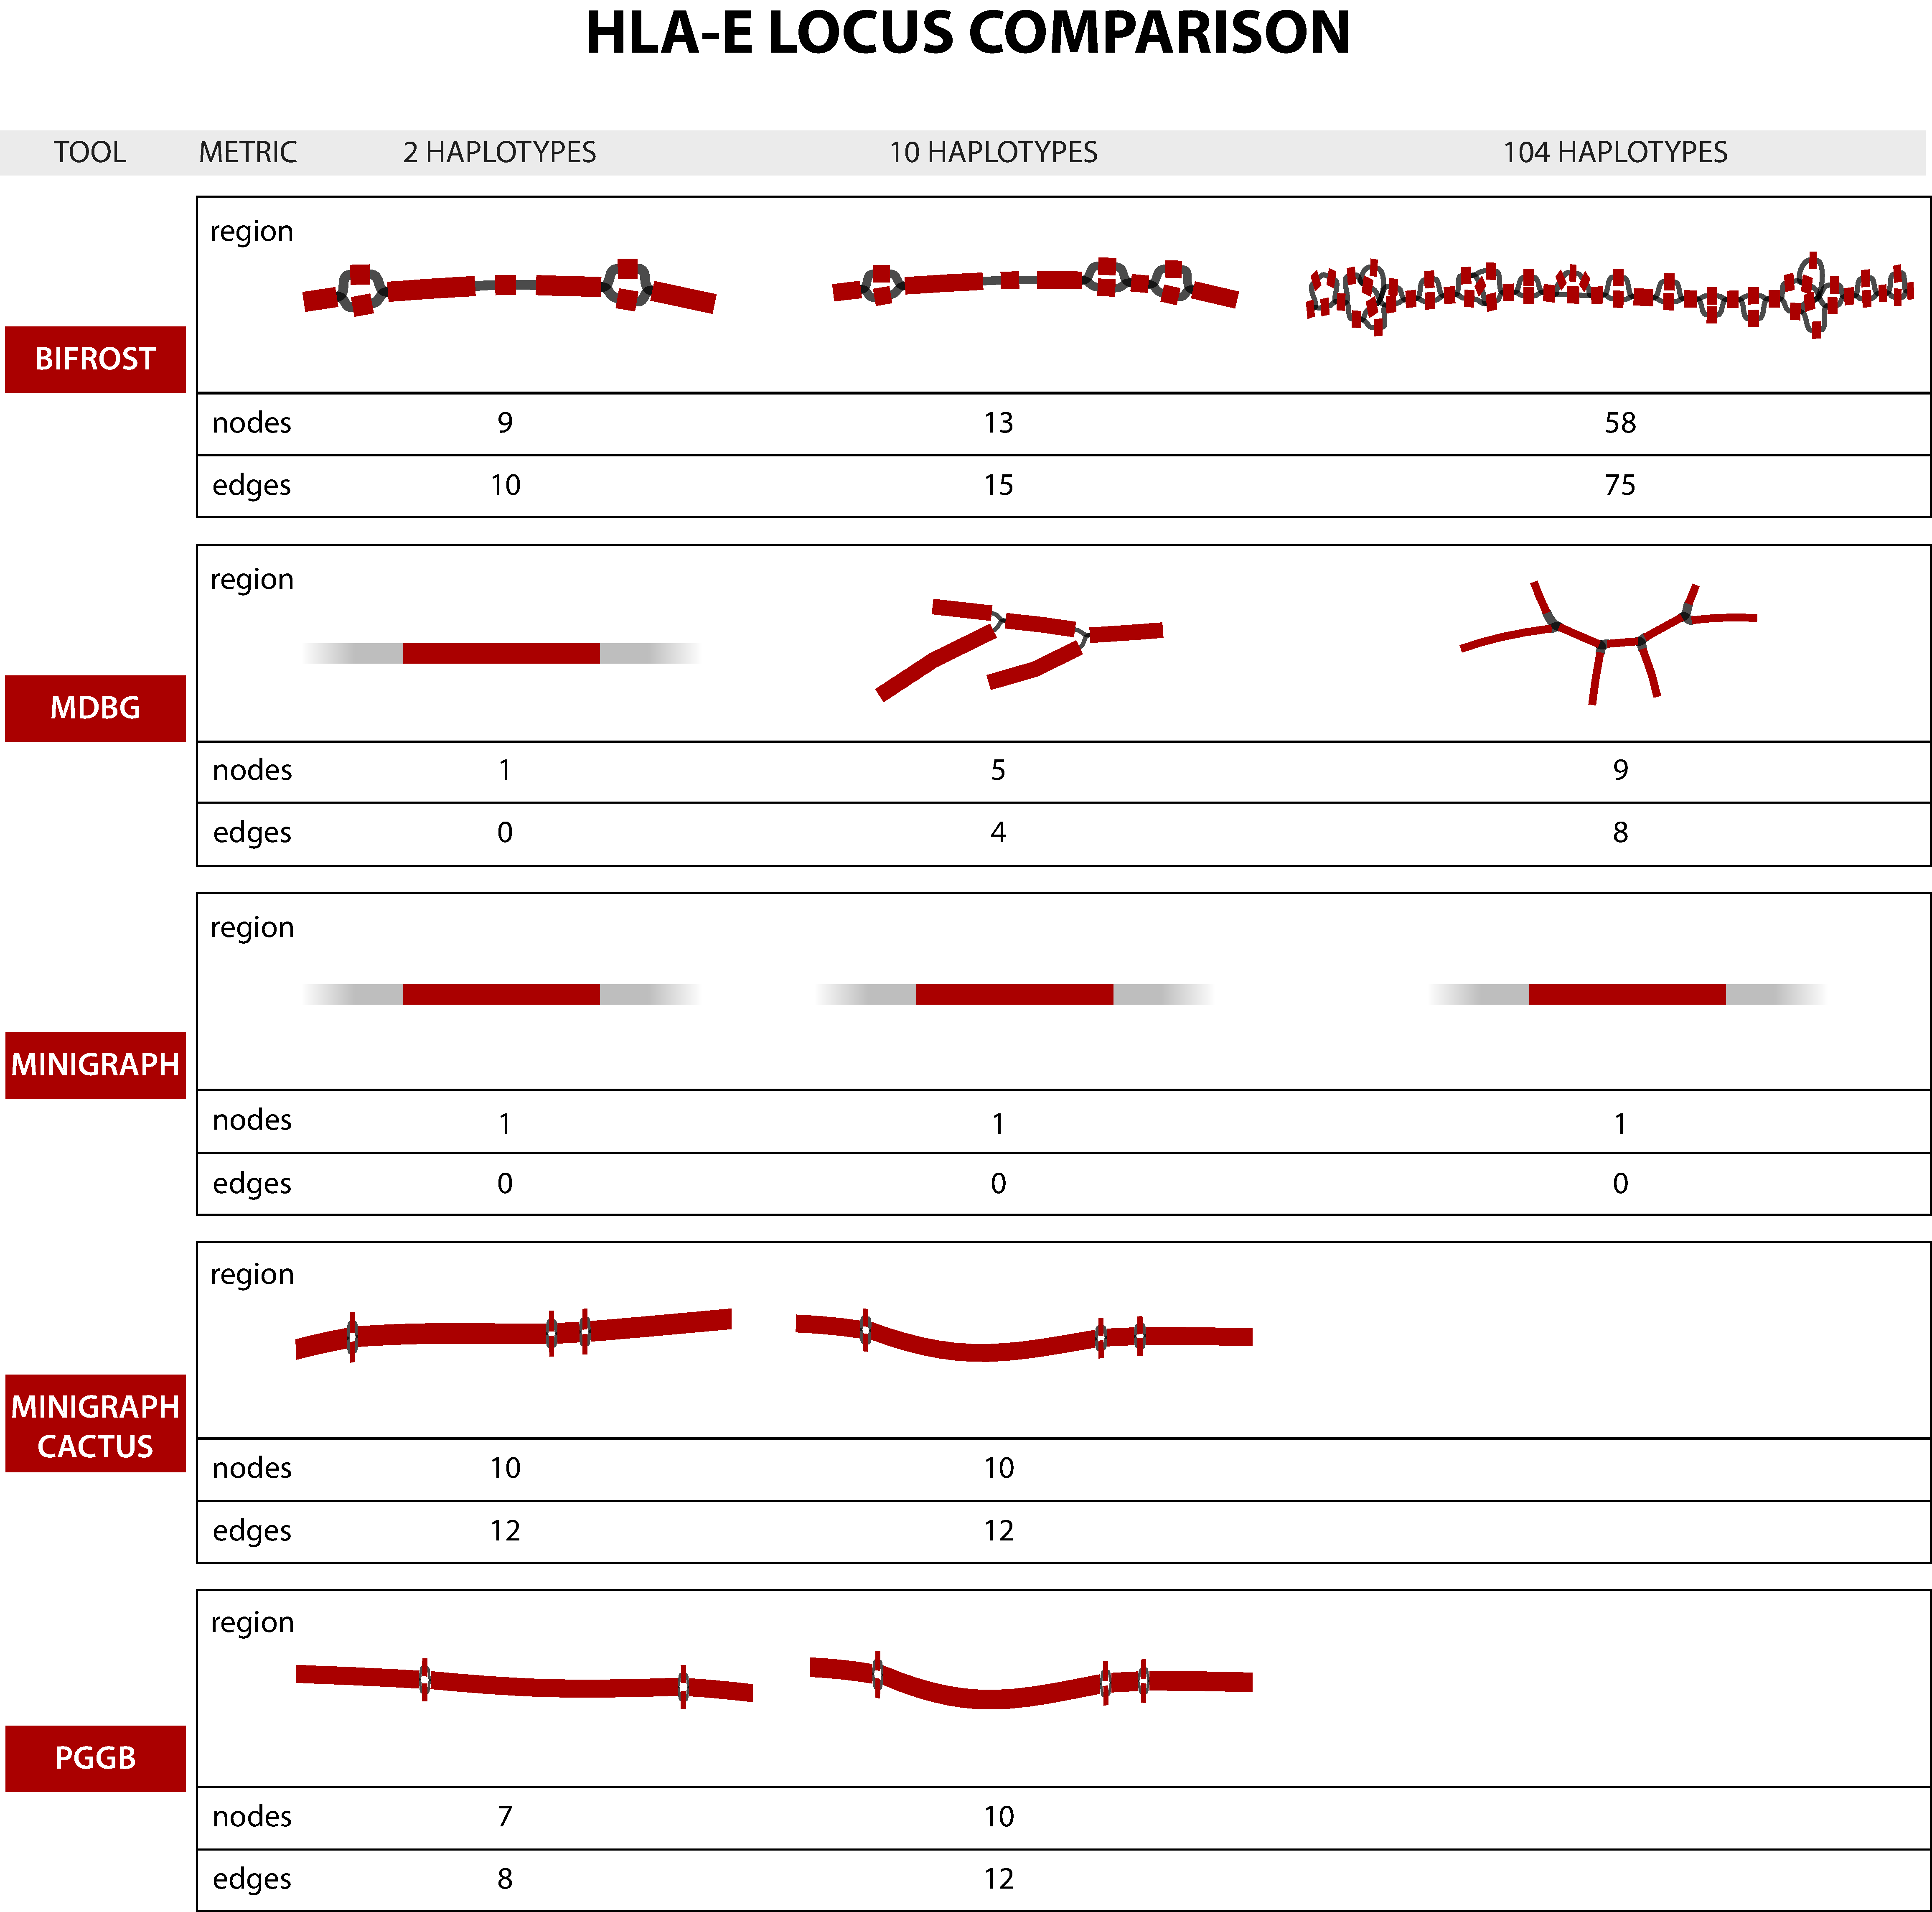
\includegraphics[width=0.95\textwidth]{figures/paperI/hla-e_corrected.pdf}
	\caption[Representations of the HLA-E locus on large human pangenomes.]{Representations of the HLA-E locus by five graph construction methods over three increasing large human pangenomes. Nodes highlighted in red contain part of the locus sequence. The numbers of nodes and edges displayed below each graph concerns the whole subgraph (both red and grey nodes). %, i.e. nodes and edges directly or indirectly attributed to the sequences that represent the locus. 
		\minigraph, on H2, H10 and H104, and \mdbg, on H2, have only a portion of one node highlighted since the 4.8k bp region is contained inside a single, long node.} 
	\label{fig:HLA-E}
\end{figure}

\paragraph{\textbf{\textup{HLA complex locus: high complexity region}}}

Figure \ref{fig:HLA-A} is the counterpart of Figure~\ref{fig:HLA-E} for the complex locus part. In this case the overall interpretability of the region is more challenging, as the number and the structure of the variations is different than in HLA-E. It is also more difficult to compare across tools. Base-level variations, e.g. SNPs, are not visually recognizable in Figure~\ref{fig:HLA-A} in the methods that retain them (i.e. \pggb, \mcactus and \bifrost) due to the large sizes of graphs.

There are notable differences in how  tools represent the variation, which is well-illustrated in the H2 dataset. While \minigraph renders H2 as a single sequence plus a large structural variant (SV) of $\approx$ 52k bp, \pggb separates it into two paths that differ by $\approx$ 54k bp in length. \bifrost represents a detailed bubble that contains many variations inside each path. In \mdbg, even extracting the complete locus is a challenge as many of the subgraph nodes were not selected by our procedure. \mcactus adds base level divergences between haplotypes on top of \minigraph SV graph.

These differences between representations are further accentuated in the H10 dataset. For it, \pggb tends to separate the haplotypes into different paths, \bifrost renders consistently the same compacted representation and \minigraph neglects most of the small differences but is able to display accurately the general picture, and \mcactus, as in H2, adds small variations on top of \minigraph structure. 


\begin{figure}[htp]
	\centering
	\includegraphics[width=0.95\textwidth]{figures/paperI/hla-a_corrected.pdf}
	\caption[Representations of the HLA-A locus on large human pangenomes.]{Representations of the complex HLA region by five graph construction methods over three increasing large human pangenomes. 
		See caption of Fig.~\ref{fig:HLA-E} for details. 
		%.Nodes highlighted in red are the ones that contain part of the locus sequence. The number of nodes and edges displayed represent the ones directly or indirectly attributed to the sequences that represent the locus.
	}
	\label{fig:HLA-A}
\end{figure}

\subsection*{\textbf{Uncovering characteristics of graphical pangenome tools}}
\label{sec:uncovering}
The data structures generated by pangenome building tools are expected to facilitate comparisons between the input genomes. In addition pangenome graphs should be stored in such a way to be easily used by downstream applications.
We identify 8 important features for pangenome graph construction tools: i) stability, ii) editability, iii) accessibility by downstream applications, iv) haplotype compression performance v) ease of visualization, vi) quality of metadata and annotation. Two other but important features, scalability and interpretability of produced graphs, were already discussed in Sections "Scalability and characteristics of pangenome graph construction tools" and "Interpretation of variation in pangenome graphs: focus on two HLA loci". %\ref{sec:scalablility} and \ref{sec:loci}. 
Table \ref{tab:tools_consideration} summarizes some of the following considerations on the relative strength of the tools.

\paragraph{\textbf{\textup{Editability and dynamic updates}}}
%\noindent\textbf{EDITABILITY AND DYNAMIC UPDATES} 
As more high quality assemblies will be generated in the near future, haplotypes may be added to a pangenome, or replaced by improved versions. Updating an existing data structure instead of rebuilding it from scratch is both computationally and energetically efficient. 
However, many succinct data structures currently used in pangenome representation are static, i.e. cannot be updated. %Current
Some methods allow a restricted set of editing operations.
\minigraph allows to add new haplotypes on top of an already built graph. \bifrost provides C++ APIs to add or remove \mbox{(sub-)sequences}, \kmers and colors from the ccdBG.
\pggb, using \odgi~\cite{odgi}, allows specific operations that delete and modify nodes and edges and add and modify paths through the graph. As \mcactus can be opened with \odgi, it supports the same operations as \pggb. 
The current \mdbg implementation uses a dynamic hash table, but does not expose an interface that supports updates.

\paragraph{\textbf{\textup{Stability}}}
%\noindent\textbf{STABILITY} 
Counter-intuitively, a pangenome graph construction tool may in some cases generate different outputs when executed multiple times with the same haplotypes as input. This \emph{unstability} could be due to a permutation in the order of the sequences given as input, or non-determinism in the construction algorithm.
Yet in order to facilitate the reproducibility of results, pangenome building tools should generate an unchanged output from the same set of input sequences, independently of the particular run or the order in which these are given.
We performed two tests to evaluate tool stability: i) we run the tools 3 times using as input the same H10 dataset and ii) we run the tools twice on shuffled input sequences, i.e. changing the order of the haplotypes of H10. 

\bifrost and \mdbg constructed exactly the same pangenome on every test, as by definition, de Bruijn graphs are stable.
\minigraph generates identical graphs on identical inputs, but generates slightly different graphs when the input is permuted. Indeed the construction algorithm of \minigraph is order-sensitive as it augments the existing graph structure by aligning the next given haplotype to it and adding divergent sequences. 
\mcactus generates slightly different graphs on identical input. 
\pggb\ generated slightly different graphs while maintaining the same haplotype sequences in the paths. The overall representation of the input genomes is therefore preserved, while the topology of the variation graph varies. The first two of the three phases of the \pggb pipeline (all-vs-all alignment and graph imputation) produce the same result on different runs with the same input but differences arise when the order of the input haplotypes changes. Most of the differences in the graph topology are thus due to the final smoothing steps.

\paragraph{\textbf{\textup{Accessibility by downstream applications}}}
% \noindent\textbf{ACCESSIBILITY BY DOWNSTREAM APPLICATION} 
\label{subs:downstream}
To facililate their adoption, pangenome representations should be easily processed by downstream analyses. 
De Bruijn graphs are challenging to analyze due to their high number of nodes, edges, and redundancy (the $k-1$-overlaps between nodes).
Though De Bruijn graph representations usually support queries of presence/absence on nodes (as in \bifrost), they lack tools able to perform more elaborate analyses such as those discussed in Section "Interpretation of variation in pangenome graphs: focus on two HLA loci", e.g. incorporating haplotype information at the \kmer level. 
On the other hand, variations graphs with paths provide more flexibility, i.e. as in \pggb and \mcactus with the \odgi visualization toolkit.
Finally in \minigraph, which considers a narrower spectrum of variants, the absence of path information prevents haplotype-level analysis; haplotypes would need to be manually mapped back to the graph. 
The choice of the pangenome building tool depends on the envisioned application. \mbox{\pggb} and \mbox{\mcactus} graphs have been shown to outperform linear references for short read mapping, genotyping and RNA sequencing mapping \mbox{\cite{hdpr}}. As these two methods  are complex pipelines based on multiple tools where parameters have been carefully set, they can be more challenging to install and run than single integrated tools. \mbox{\minigraph} alone can also be used if the focus is on structural variation instead of SNPs or small indels, and to quickly produce a pangenome graph for complex loci visualization and interpretation. The dBG-based approaches show that, for example with \mbox{\bifrost}, they retain the same base-level information as more computational-heavy variation graph approaches, but the lack of tools to use them for analysis limits their adoption.

\paragraph{\textbf{\textup{Haplotype compression}}}
%\noindent\textbf{HAPLOTYPE COMPRESSION} 
Building a graph pangenome can be seen also as a way to store, compact and retrieve the input haplotypes. As the number of new assemblies is growing faster than the data storing capacity, pangenomes can potentially help save storage space. This is highlighted by the disk space reported in Table~\ref{tab:computational_metrics}, which is consistently smaller than the sum of haplotype sizes for all methods and datasets.

In order to losslessly retrieve the input genomes from a pangenome, the  representation has to store all variations from the original haplotype sequences as paths in the graph. \pggb and \mcactus fall into this category while the other three considered tools do not store paths, or do not consider all variations, thus they are lossy.

Of note, the GBZ tool~\cite{gbz} enables graph pangenomes that store paths in the GFA file format %(the consensus file format used) 
to be stored in a lossless compressed form. It uses a Graph Burrows-Wheeler transformation to compress the graph in a more efficient way than using gzip~\cite{gbz}. Using GBZ, the pangenomes generated by \pggb and \mcactus are losslessly compressed with space gains of 3.5-5x.


\paragraph{\textbf{\textup{Ease of Visualization}}}
%\noindent\textbf{EASE OF VISUALIZATION} 
Visualizing large graphs which exceed hundreds of thousands of node is a challenge that exceeds the scope of pangenomics. The H104 pangenomes  are difficult to visualize.
Among the visualization tools considered by the Human Pangenome Reference consortium~\cite{hpp}, 
only \bandage is able to display the \minigraph or \mdbg H104 graphs, which contains a few million nodes. We reduced the number of nodes and edges of \pggb, \mcactus and \bifrost H10 graphs by collapsing isolated subgraphs representing SNPs or indels up to 10k bp (using the command \texttt{gfatools asm -b 10000 -u}). % to be able to display them. 
%Generally, general-purpose graph drawing tools able to visualize graphs with millions of nodes are needed, in particular to extract and display specific loci.

\paragraph{\textbf{\textup{Quality of Metadata and Annotation}}}
%\noindent\textbf{QUALITY OF METADATA AND ANNOTATION} 
Augmenting pangenome structures with information from other omics data would increase pangenome relevance in biological discoveries. As biobanks are rapidly growing, more data is available on regulatory regions, transcriptomics, CNVs and other medically relevant traits~\cite{100000genomes,ucla}. Pangenome data structures could leverage such information, and some of the considered tools offer basic functionality in this sense.
\bifrost provides a function to link data to graph vertices through C++ APIs. \pggb and \mcactus, using \odgi, offer annotation capabilities through insertion of paths or BED records. \minigraph and \mdbg do not offer any annotation feature. 
Specifically, in order to enhance a pangenome graph with metadata (for example with genes and regulatory regions known variants), it is desirable to maintain compatibility with methods and data formats that use a linear reference. One could conceivably project data from a graph to a reference genome to continue downstream analyses using linear coordinates. A simple method to achieve this compatibility, in our view, is to store the reference genome of interest inside the graph pangenome that supports retrieving such a reference. Variation graphs built using \mbox{\pggb or \mcactus}, due to their locally acyclical and directed construction and their use of haplotype paths, store all the coordinates needed for such a task. Haplotype paths play an important role as they avoid additional mapping to the graph, by using the \mbox{\odgi}tool to extract or inject the required information. \mbox{\minigraph} does not store haplotype paths and requires mapping sequences to the graph to restore haplotype information. On the other hand, De Bruijn graphs, using associated color data, can record the membership of k-mers to a reference sequence, yet one cannot fully reconstruct a haplotype unless k-mers positions are also stored.
\begin{table}
	\centering
	\caption[Relative strengths of five pangenome graph construction tools.]{\textbf{Relative strengths of five pangenome graph construction tools}\\
		Explanation of rows:
		1) efficacy of construction algorithm, measuring wall-clock time;
		2) degree to which variants (e.g. SNPs) are retained;
		3) ability of a tool to perform well on large datasets, both in comparison to other tools but also compared to smaller datasets;
		4) ability to modify the produced data structure to add or remove haplotypes; 
		5) property of producing the same result irrespective of perturbations, such as permutation of the input order, and repeating the same run;
		6) existence of tools (and operations) that can be applied to the resulting graphs; 
		7) whether input haplotypes information is retained by the tools, and if so, its space efficiency;
		8) whether the entire graph can be directly visualized and interpreted; 
		9) easiness of 'zooming in' a specific genomic region and interpret variants;
		10) summarizes the functionalities provided by the tools to annotate the pangenomes with genomic data;
		11) ability to share information between the graph and a linear reference.
	}
	\resizebox{\textwidth}{!}{
		\begin{tabular}{|l c c c c c|} 
			\hline
			Metric & \bifrost & \pggb & \mcactus & \minigraph & \mdbg\\
			\hline
			1) Construction speed & $\bullet\bullet\circ$ & $\bullet\circ\circ$ & $\bullet\circ\circ$ &  $\bullet\bullet\circ$ & $\bullet\bullet\bullet$\\
			\hline
			2)  Variations & $\bullet\bullet\bullet$ & $\bullet\bullet\bullet$ & $\bullet\bullet\bullet$ & $\bullet\bullet\circ$ & $\bullet\bullet\circ$\\
			\hline
			3) Scalablilty & $\bullet\bullet\bullet$ & $\bullet\circ\circ$ & $\bullet\circ\circ$ & $\bullet\bullet\circ$ & $\bullet\bullet\bullet$\\
			\hline
			4) Editability & $\bullet\bullet\bullet$ & $\bullet\bullet\circ$ & $\bullet\circ\circ$ & $\bullet\bullet\circ$ & $\bullet\circ\circ$\\
			\hline
			5) Stability & $\bullet\bullet\bullet$ & $\bullet\circ\circ$ & $\bullet\circ\circ$ & $\bullet\bullet\circ$ & $\bullet\bullet\bullet$\\
			\hline
			6) Accessibility by downstream applications & $\bullet\circ\circ$ & $\bullet\bullet\bullet$ & $\bullet\bullet\bullet$ & $\bullet\bullet\circ$ & $\bullet\circ\circ$\\
			\hline
			7) Haplotype compression performance & $\bullet\bullet\circ$ & $\bullet\bullet\bullet$ & $\bullet\bullet\bullet$ & $\bullet\circ\circ$ & $\bullet\circ\circ$\\
			\hline
			8) Ease of visualization  & $\bullet\circ\circ$ & $\bullet\bullet\circ$ & $\bullet\bullet\circ$ & $\bullet\bullet\bullet$ & $\bullet\bullet\bullet$ \\
			\hline
			9) Loci visualization and interpretability   & $\bullet\circ\circ$ & $\bullet\bullet\circ$& $\bullet\bullet\bullet$ & $\bullet\bullet\circ$  & $\bullet\circ\circ$\\
			\hline
			10) Metadata and annotation   & $\bullet\bullet\circ$ & $\bullet\bullet\bullet$ & $\bullet\bullet\circ$ & $\bullet\circ\circ$  & $\bullet\circ\circ$\\
			\hline
			11) Compatibility with a linear reference coordinates & $\bullet\circ\circ$ & $\bullet\bullet\bullet$ & $\bullet\bullet\bullet$ & $\bullet\bullet\circ$  & $\bullet\circ\circ$\\
			\hline
	\end{tabular}}
	\label{tab:tools_consideration}
\end{table}

\section{Discussion}
Five state-of-the-art pangenome graphs construction tools were compared on the representation of up to 104 human haplotypes. The approaches significantly differ in terms of speed, graph size, and representation of variations. We find that it remains computationally prohibitive to generate human pangenome graphs for hundreds of haplotypes, especially while retaining all variations. Each approach has its own set of strengths, and ultimately the choice of the method depends on the downstream application. In addition, several takeaway points emerged from our analysis.

First, our focused analysis of HLA loci revealed that de Bruijn graphs and variation graphs represent genomic variations equally well as pangenomes.  This is of particular importance as also shown by the draft human pangenome references~\mbox{\cite{hdpr}}: pangenomes are pivotal to trace complex and clinically relevant loci. While de Bruijn graphs are faster to construct, more stable, and scale better in terms of input size, the resulting graphs are challenging to interpret downstream. Variations graphs on the other hand are more practical to analyze at the expense of a less efficient construction step. Their visualization are more straightforward to interpret, mostly due to not having cycles, and provide insights into loci differences. 

Second, we can highlight two categories of pangenomic methods that have distinct application domains. \pggb, \mcactus and \bifrost store all possible variations, and keep haplotype information as paths or colors. They provide a complete picture of the set of variations in the input genomes which makes them difficult to analyze. They can be used for a large variety of genomic analysis, as shown for \mbox{\pggb} and \mbox{\mcactus}~\mbox{\cite{hdpr}}. \minigraph and \mdbg generate 'sketched' pangenome graphs that consider only large variants, ignoring smaller differences, and are more efficient to construct and visualize. They can be used for large scale characterization of variation in population, as proven for bacteria \mbox{\cite{mdbg}}.

Third, every tool possesses an exclusive set of features.
\pggb facilitates downstream analyses using the companion tool \odgi. It allows to precisely extract and browse any locus of interest. It is the only tool that generates variation graphs without a reference. It also keeps a lossless representation of the input sequences.
\minigraph generates a pangenome graph based on a reference sequence taken as a backbone. Its shines in the representation of complex structural variations, but does not include small or inter-chromosomal variations.
The pipeline \mcactus, that uses the \cactus base aligner, can be used to add small level variations on top of the \minigraph graph and to keep a lossless representation of the input sequences.
\bifrost illustrates that classical de Bruijn graphs are scalable, stable, dynamic, and store all variations. However, extracting information from them remain a challenge.
Lastly, \mdbg\ is the fastest construction method which generates an approximate representation of differences between haplotypes. As discussed in Section "Accessibility by downstream applications", these features enable different genomic analyses and downstream applications.

\section{Conclusions}
In conclusion, our results highligh the strengths and weaknesses of current pagnenome construction tools for human applications, with specific focus on how do they represent specific loci of medical relevance. We also provide insights on the features they possess and point out their best application domains.
In our view, future directions for human pangenomes building tools should focus on tackling efficiency bottlenecks, aiming to represent hundreds to thousands of haplotypes. Representations should further be lossless and represent the input haplotypes as paths in the graph. 
Such features would unlock many other applications such as lossless compression of haplotypes and cancer copy number variant analysis. 
Finally, we recognize the need for more user-friendly tools that can be used by biologists and that can translate complicated questions into  graph queries. While \odgi begins to address these questions in variation graphs, other approaches have not yet provided user-friendly interfaces. A package similar to \odgi for de Bruijn graphs would help fully realize their potential.

\section{Methods}
\subsection*{\textbf{Datasets and haplotypes collection}}
\label{sec:datasets}
In order to evaluate the state of current human pangenome representations, we sought to build a human pangenome that contains all publicly available high-quality human haplotypes. We collected from two different sources 102 different haplotypes from the genome of 51 individuals, and also used the two reference genomes, GRCh38 from the Genome Reference Consortium (GRC) \cite{grc} and CHM13 v2.0 cell line of the T2T Consortium~\cite{t2t}.
Five haplotypes correspond to Google Brain Genomics DeepConsensus \cite{deepconsensus} assembly dataset: they are hifiasm assemblies of PacBio Hi-Fi reads corrected with DeepConsensus. The average of their N50 is 37,99 Mbp. 
The remaining haplotype assemblies as well as the T2T reference are from the Human Pangenome Reference Consortium (HPRC) year-1 freeze~\cite{hpp}, and GRCh38 is from the GRC. Their average N50 is 40.3 Mbp. Since HG002 is contained in the DeepConsensus data, the HPRC HG002 haplotypes were not used.
The origin and the sex of the individuals are diverse %to aim for a 
and provide a fair representation of the diversity in human population: out of 51 total individuals, 21 are males and 30 are females and they represent 14 different ethnic groups, from US to Africa and Asia. We did not perform any additional selection, regarding sex and ethnicity, on these public datasets as our main goal was to use as many genomes as possible. However, the HPRC stated that the genomes were selected to represent genetic diversity in humans~\mbox{\cite{hdpr}}.

To evaluate the scalability of pangenome construction tools, we created three datasets of increasing size: 1) 2 haplotypes from the same individual, HG006, 2) 10 haplotypes from 5 different individuals (HG002, HG003, HG004, HG006 and HG00735) and finally 3) all of the 104 haplotypes. To test whether the order of the input sequences matters, we considered various random orderings for the 10 haplotypes in Dataset 2. Since \minigraph needs a reference sequence as fist haplotype in order to correctly build the graph, we generated specific 2 and 10 haplotypes datasets with the first haplotype replaced by the reference genome CHM13. This was applied to the \mcactus pipeline as well as it uses \minigraph variation graphs.

\begin{table}
	\centering
	\setlength{\tabcolsep}{5pt} 
	\caption[Description of the three datasets generated to test the scalability of the tools.]{\textbf{Description of the three datasets generated to test the scalability of the tools}
		\\
		Data sources: 
		$^1$ Google Brain Genomics~\cite{google-assemblies}; $^2$ Human Pangenome Reference Consortium~\cite{HPRC-haplotypes}; $^3$ 1000 Genomes Project~\cite{HPRC-haplotypes}; $^4$ Telomere to Telomere Consortium~\cite{HPRC-haplotypes}.
		\label{tab:datasets}}
	\renewcommand{\arraystretch}{1.2}
	\begin{tabular}{|c c c|}
		\hline
		\centering
		Haplotypes & Project & Bases \\
		\hline
		2 & Google$^1$ & 5.9 Gbp\\
		10 & Google, HPRC$^2$ & 30 Gbp \\
		104 & Google, HPRC, 1KG$^3$, T2T$^4$ & 313.6 Gbp \\
		\hline
	\end{tabular}
\end{table}

\subsection*{\textbf{Pangenome graph construction tools}}
\label{sec:tools}

We evaluated tools that generate graph pangenomes as variation graphs and colored compacted de Bruijn graphs. Variation graphs are generally locally acyclic while de Bruijn graphs have cycles. In variation graphs, nodes represent sequences and edges represent immediate sequence adjacency without overlap. Variation graphs are generally easier to visualize and to interpret while challenging to construct at scale and, apart from \pggb, require a reference genome. In de Bruijn graphs (\dbg), nodes are \kmers (string of length k) and edges are (k-1)-overlaps between nodes. In practice, \dbgs are represented in a compact way where all nodes along unbranching paths are compacted into \emph{unitigs}. The resulting graph is called compacted De Bruijn Graph, where nodes are unitigs and edges represent (k-1)-overlaps. 
As shown in Figure \ref{fig:figure1}, de Bruijn graphs %are easier to construct and are more standardized but 
result in large graphs that pose visualization and interpretation challenges, in particular as there is no alignment to a reference.

\begin{itemize}
	\item
	\bifrost constructs dynamic, coloured compacted de Bruijn Graphs (\emph{\ccdbg}). It first generates a standard \dbg using an efficient variant of Bloom Filters and then computes the compacted \dbg from it.
	Colors, i.e. identifiers representing the sample origin of each k-mer are added by storing an array per \kmer. A human genome \ccdbg typically consists of a single large connected component, as common \kmers are shared between chromosomes. This pangenome representation contains all the variations present in input sequences.
	
	\item
	\mdbg builds a variant of de Bruijn graphs called a minimizer-space de Bruijn Graph (\mdbg), which is efficient to construct as it only considers a small fraction of the input nucleotides. Color information is currently not supported in the implementation. Similarly to Bifrost, a \mdbg also typically represents a human genome as a single large connected component, albeit with orders of magnitude less nodes. Minimizer-space de Bruijn graphs mostly discard small variants, yet are sensitive to heterozygosity which creates branches in the graph.
	
	\item
	\minigraph constructs a directed, bidirected and acyclic variation graph iteratively by mapping new haplotypes using a combination of the minimap2 tool and the graph wavefront alignment algorithm. The first input sequence acts as a  backbone for the whole representation.
	The sample(s) of each node are stored in a rGFA output file.
	\minigraph considers only variations longer than 50 bps hence it is oblivious to isolated SNPs and small indels: even if it produces base-level alignment for contigs, the graphs are not a base-level resolution. The resulting graph is divided into connected components that correspond to the chromosomes present in the first given input genome.
	%, yet can represent large divergent regions at base-pair resolution
	\item
	\mcactus is a variation graph construction pipeline that combines \minigraph to generate a structural variations graph and \cactus base aligner to generate base-level pangenome graphs of a set of input assemblies and embg: The definition of \label has changed! Check your packages! Replacing it with the kernel definition on input line 145.ed haplotypes paths. \cactus~\cite{cactus} is a highly accurate and scalable reference-free multiple whole-genome alignment tool, that in this pipeline considers the reference sequence used by \minigraph to ensure that the resulting variation graph is acyclic. The final graph is further normalized using GFAffix\cite{gfaffix}. The pipeline allows to generate multiple graphs, one for each chromosome, or produce a single graph that includes inter-chromosomal variants.
	
	\item
	\pggb is a directed acyclic variation graph construction pipeline rather than a single tool. It calls three different tools: pairwise base-level alignment  of haplotypes using wfmash \cite{wfmash}, graph construction from the alignments with seqwish \cite{seqwish}, graph sorting and normalization with smoothxg and GFAffix \cite{smoothxg,gfaffix}.
	The resulting variation graph represents variations of all lengths present in the input sequences.
\end{itemize}


\begin{table}
	\centering
	\caption[URL, version, pangenome representation and parameters of the three analyzed tools.]{ \textbf{URL, version, pangenome representation and parameters of the three analyzed tools.}\\ pggb/0.2.0 used wfmash v0.7.0, seqwish v0.7.3 and smoothxg v0.6.1.}
	\resizebox{\textwidth}{!}{
		\begin{tabular}{|c c c c c|} 
			\hline
			Tool  &  Github repository & Graph type & Version & Parameters \\ 
			\hline \hline
			\bifrost & pmelsted/Bifrost  & De Bruijn graph  & 1.0.5 & -k100 -c \\ 
			\hline
			\pggb &   pangenome/pggb & variation graph  & 0.2.0 & -p 98 -s 10000 -k 311 -G 13033,13117\\ &&&& -O 0.03 -v -t 8 -T 8 -A -Z \\ 
			\hline
			\minigraph & lh3/Minigraph  & variation graph &   0.18 & -cxggs\\ 
			\hline
			\mcactus & ComparativeGenomics  & variation graph &   2.2.3 & --maxLen 10000 --delFilter 10000000 \\ & Toolkit/cactus &&&\\ 
			\hline
			\mdbg  & ekimb/rust-mdbg  & De Bruijn graph &  1.0.1 & -k 10 -d 0.0001 --minabund 1 --reference\\ 
			\hline
	\end{tabular}}
	\label{tab:url}
\end{table}



\section*{Supplementary Information}

\subsection*{\textbf{Benchmark infrastructure}}

Running time of pangenome construction tools was measured as wall clock time and peak memory as maximum resident set size using the \texttt{time} command. Other metrics were obtained with custom Python scripts. All benchmarks were performed on a Supermicro Superserver SYS-2049U-TR4, with 3 TB RAM and 4 Intel SKL 6132 14-cores @ 2.6 GHz, using 8 cores. \\

\subsection*{\textbf{TwoPaCo}}
\label{app:twopaco}
We did not consider \twopaco as it is redundant with \bifrost. Both methods construct the same de Bruijn graphs.
\twopaco is a method for constructing \ccdbgs by finding junction \kmers at the boundaries of unitigs or in branching nodes. It consists of two main steps in which it approximates the dBG with a Bloom filter in order to reduce the size of the problem and then runs a two pass highly parallel algorithm on it. It constructs ccdBGs similarly to \bifrost. \bifrost  is faster, supports edit operations, and accepts also reads other than assemblies as input. We tested both tools on NCBI datasets from three different known human variation regions part of the human leukocyte antigen (HLA) complex: HLA-A, MICB and TAP1. These loci have different number of sequences and have complexity and length. The resulting graphs have exactly the same k-mer content and substantially equal topology. The difference is that \twopaco considers sequences with IUPAC 'N' bases while \bifrost does not and that in some cases \twopaco renders some unitigs split in two or more consecutive nodes.

\subsection*{\textbf{Loci extraction method}}
\label{app:extraction}
For \bifrost and \mdbg graphs, nodes corresponding to the input sequences are identified with \graphaligner\cite{graphaligner} and the subgraph is extracted using the \bandage \emph{reduce} function. As the aligned nodes are not expected to represent the full diversity of the population in the pangenomes, the considered portion of the graph contains also nodes up to a certain distance from the aligned ones: 1 for \mdbg and 3 for \bifrost. This number is based on the size of the sequences spelled by the nodes and on the considered variations. Artifacts, mostly tips, that are not part of the locus of interest are removed with a custom python script. For \minigraph generated graphs, the \minigraph own alignment function has been used to identify the nodes and then \bandage is used to extract the subgraph. For \pggb, first we generate a bed file of the position of the region of interest in every haplotype used to construct the graph. The ranges are derived from aligning them to the locus sequence(s) using minimap2 \cite{minimap2}. The graph corresponding to the region is then extracted using the \odgi extract and \odgi view functions. For \mcactus we use the same strategy as \pggb, with the difference that the bed file is only for the reference CHM13, present in the graph. \\
The annotation of the specific loci in the subgraph is done using nodes from the alignment with \minigraph or \graphaligner to the subgraph. This makes it possible to highlight multiple sections in the region, as, for example, genes and pseudogenes of interest. 

\section*{\textbf{Availability of data and materials}} %Reproducibility and Data Availability
The scripts used to generate and analyse the pangenomes can be found at \cite{source-code-github}\cite{source-code-zenodo} under MIT license.
Google Brain Genomic assemblies can be found at \cite{google-assemblies}. \\
HPRC assemblies, CHM13 and GRCh38 can be found at \cite{HPRC-haplotypes}.

\section*{\textbf{Funding}}
R.C was supported by ANR Full-RNA, SeqDigger, Inception and PRAIRIE grants (ANR-22-CE45-0007, ANR-19-CE45-0008, PIA/ANR16-CONV-0005, ANR-19-P3IA-0001). This project has received funding from the European Union’s Horizon 2020 research and innovation programme under the Marie Skłodowska-Curie grants agreements No. 872539 and 956229.

\section*{\textbf{Author's contributions}}
FA, YD and RC conceived and designed the project. FA implemented the scripts. FA and PL ran the experiments. FA, YD, PL and RC wrote the paper. The authors read and approved the final manuscript.

%% Format bibliography like a section, not a chapter:
% \printbibliography[heading = subbibliography]
% \stopcontents[chapters]© Francesco Andreace, 2024

Series of dissertations submitted to the
Insitut Pasteur Paris, Universite’ de Paris Cite, University of Oslo
No. 1234
ISSN 1234-5678
All rights reserved. No part of this publication may be
reproduced or transmitted, in any form or by any means, without permission

\paragraph{Authors' affiliations}
\begin{description}
	\item[Francesco Andreace]
	Institut Pasteur, Université Paris Cité, G5 Sequence Bioinformatics \\
	Sorbonne Université, Collège doctoral \\
	25-28 Rue du Dr Roux, 75015 Paris
	
	
	\item[Pierre Lechat]
	Bioinformatics and Biostatistics Hub, Institut Pasteur, Université de Paris Cité \\
	25-28 Rue du Dr Roux, 75015 Paris
	
	\item[Yoann Dufresne]
	Institut Pasteur, Université Paris Cité, G5 Sequence Bioinformatics \\
	Bioinformatics and Biostatistics Hub, Institut Pasteur, Université de Paris Cité \\
	25-28 Rue du Dr Roux, 75015 Paris
	
	\item[Rayan Chikhi]
	Institut Pasteur, Université Paris Cité, G5 Sequence Bioinformatics \\
	25-28 Rue du Dr Roux, 75015 Paris
\end{description}
\newpage

\section{Perspectives}
The results of the work outlined in this section suggest several directions for future investigation and software development: they can be divided into a few axis.
On one side, the scripts and software that I developed to produce the analysis of this paper could have been extended into an automatic reproducible pipeline. By integrating the code into platforms like nextflow or Snakemake, this could become a benchmark for current and future pangenome tools, as, at the moment, there is no other way to independently compare the output of tools that produce variation graphs and \dbgs. \\
On another side, there are many more features that could be added to the analysis workflow to produce a more in-depth and accurate description of the resulting pangenomes, like node (sequence) length distribution, node degree distribution, count of SNPs and indels. It is important to stress that detection of specific pattern of variation is non-trivial in data-structures like \dbgs. Finally, another experiment that could be done is to convert, using path information, the variation graph into a \ccdbg, to compare against a \ccdbg built directly from the input sequences: this would allow to verify if the information stored into the two data structures is equivalent. \\
Another very interesting avenue would be to develop a tool that enables complex information extraction from \ccdbgs. Construction tools usually offer commands or apis to perform simple absence/presence queries, that are mostly useful when they are used for metagenomic purposes but offer less actionable insight in pangenomics analysis. An idea that I have started exploring during this PhD is to extract a subgraph of a \ccdbg that represent a locus or gene of interest in the whole dataset provided as input. \\ 
Finally, it would be very useful to define a \ccdbg output color format that every tool should also use to output the colors, like gfa is used to output graphs. As of now, each tool implements its own binary format for color storage, discouraging downstream analysis software development, as it would be bound to specific construction tools and not the common data structure used.

\newpage

\section{Building a \emph{Lodderomyces elongisporus} pangenome reference: overcoming current limitations.}
Here we present another example of pushing the boundaries of variation graph pangenome building strategies, precisely in producing a graph that can represent inter-chromosomal events, like rearrangements, for the medically interesting yeast strain of \lodelo. We show also how a pangenome based approach can help produce a more comprehensive insight of such events than a linear genome based one.\\
The work presented here is also in part a team effort with other PhD students and researcher I was co-leading with Daniel Doerr during a winter-school organized by my consortium: Simon Heumos, which I would like to thank for the discussion we had on the construction of such graphs and Nicola Rizzo. Most of the results and findings reported here are moslty my own, subsequent, work.\\
The following sections will explain the process needed to produce custom, biologically-significant and biologically-driven pangenome graphs of a yeast strain with the current state-of-the-art tools and offer insights on workarounds that can be used in cases with special needs, where current tools features limit the analysis that can be done. This will also show how pangenome models can offer more powerful tools to analyze specific variation in a group of similar genomes compared to linear reference based ones.\\ 
In this specific case, the goal was to produce a variation graph that considered, and showed, the long chromosomal translocations that were noticed by the team that produced the assemblies from short and long reads. Chromosome-crossing syntenies for multiple contigs in alignment hits of chromosomes C, G, and H, were detected, suggesting that they could correspond to a singular same recombination group. This finding was consistent with an independent SNP-based genomic study. It was performed on the isolates of a fungemia outbreak in a neonatal intensive care unit in Delhi between 2021 and 2022 and it noticed that this translocation events are more frequent in hospital and patient associated populations than in fruit ones~\cite{lodelo_india}. \\
In summary, the work here presented will be organized as follows:
\begin{enumerate}
	\item Brief characterization of \lodelo genome and relevance;
	\item Pangenome graphs constructed and their utility;
	\begin{enumerate}
		\item Determining the chromosomal communities from the assemblies to generate a variation graph of interest;
		\item Producing a variation graph with \pggb;
		\item Producing a variation graph with \mcactus by customizing the pipeline and the data;
	\end{enumerate}
	\item Representation of translocation events in variation graphs;
\end{enumerate}

%By plotting the alignments of the 2 best quality assemblies, B2 and J2, for chromosome C,G and H, shown in figure~\ref{fig:lodelo_dotplot-alignments}.
%\begin{figure}[t]
%	\centering
%	\begin{subfigure}[b]{0.46\textwidth}
%		\centering
%		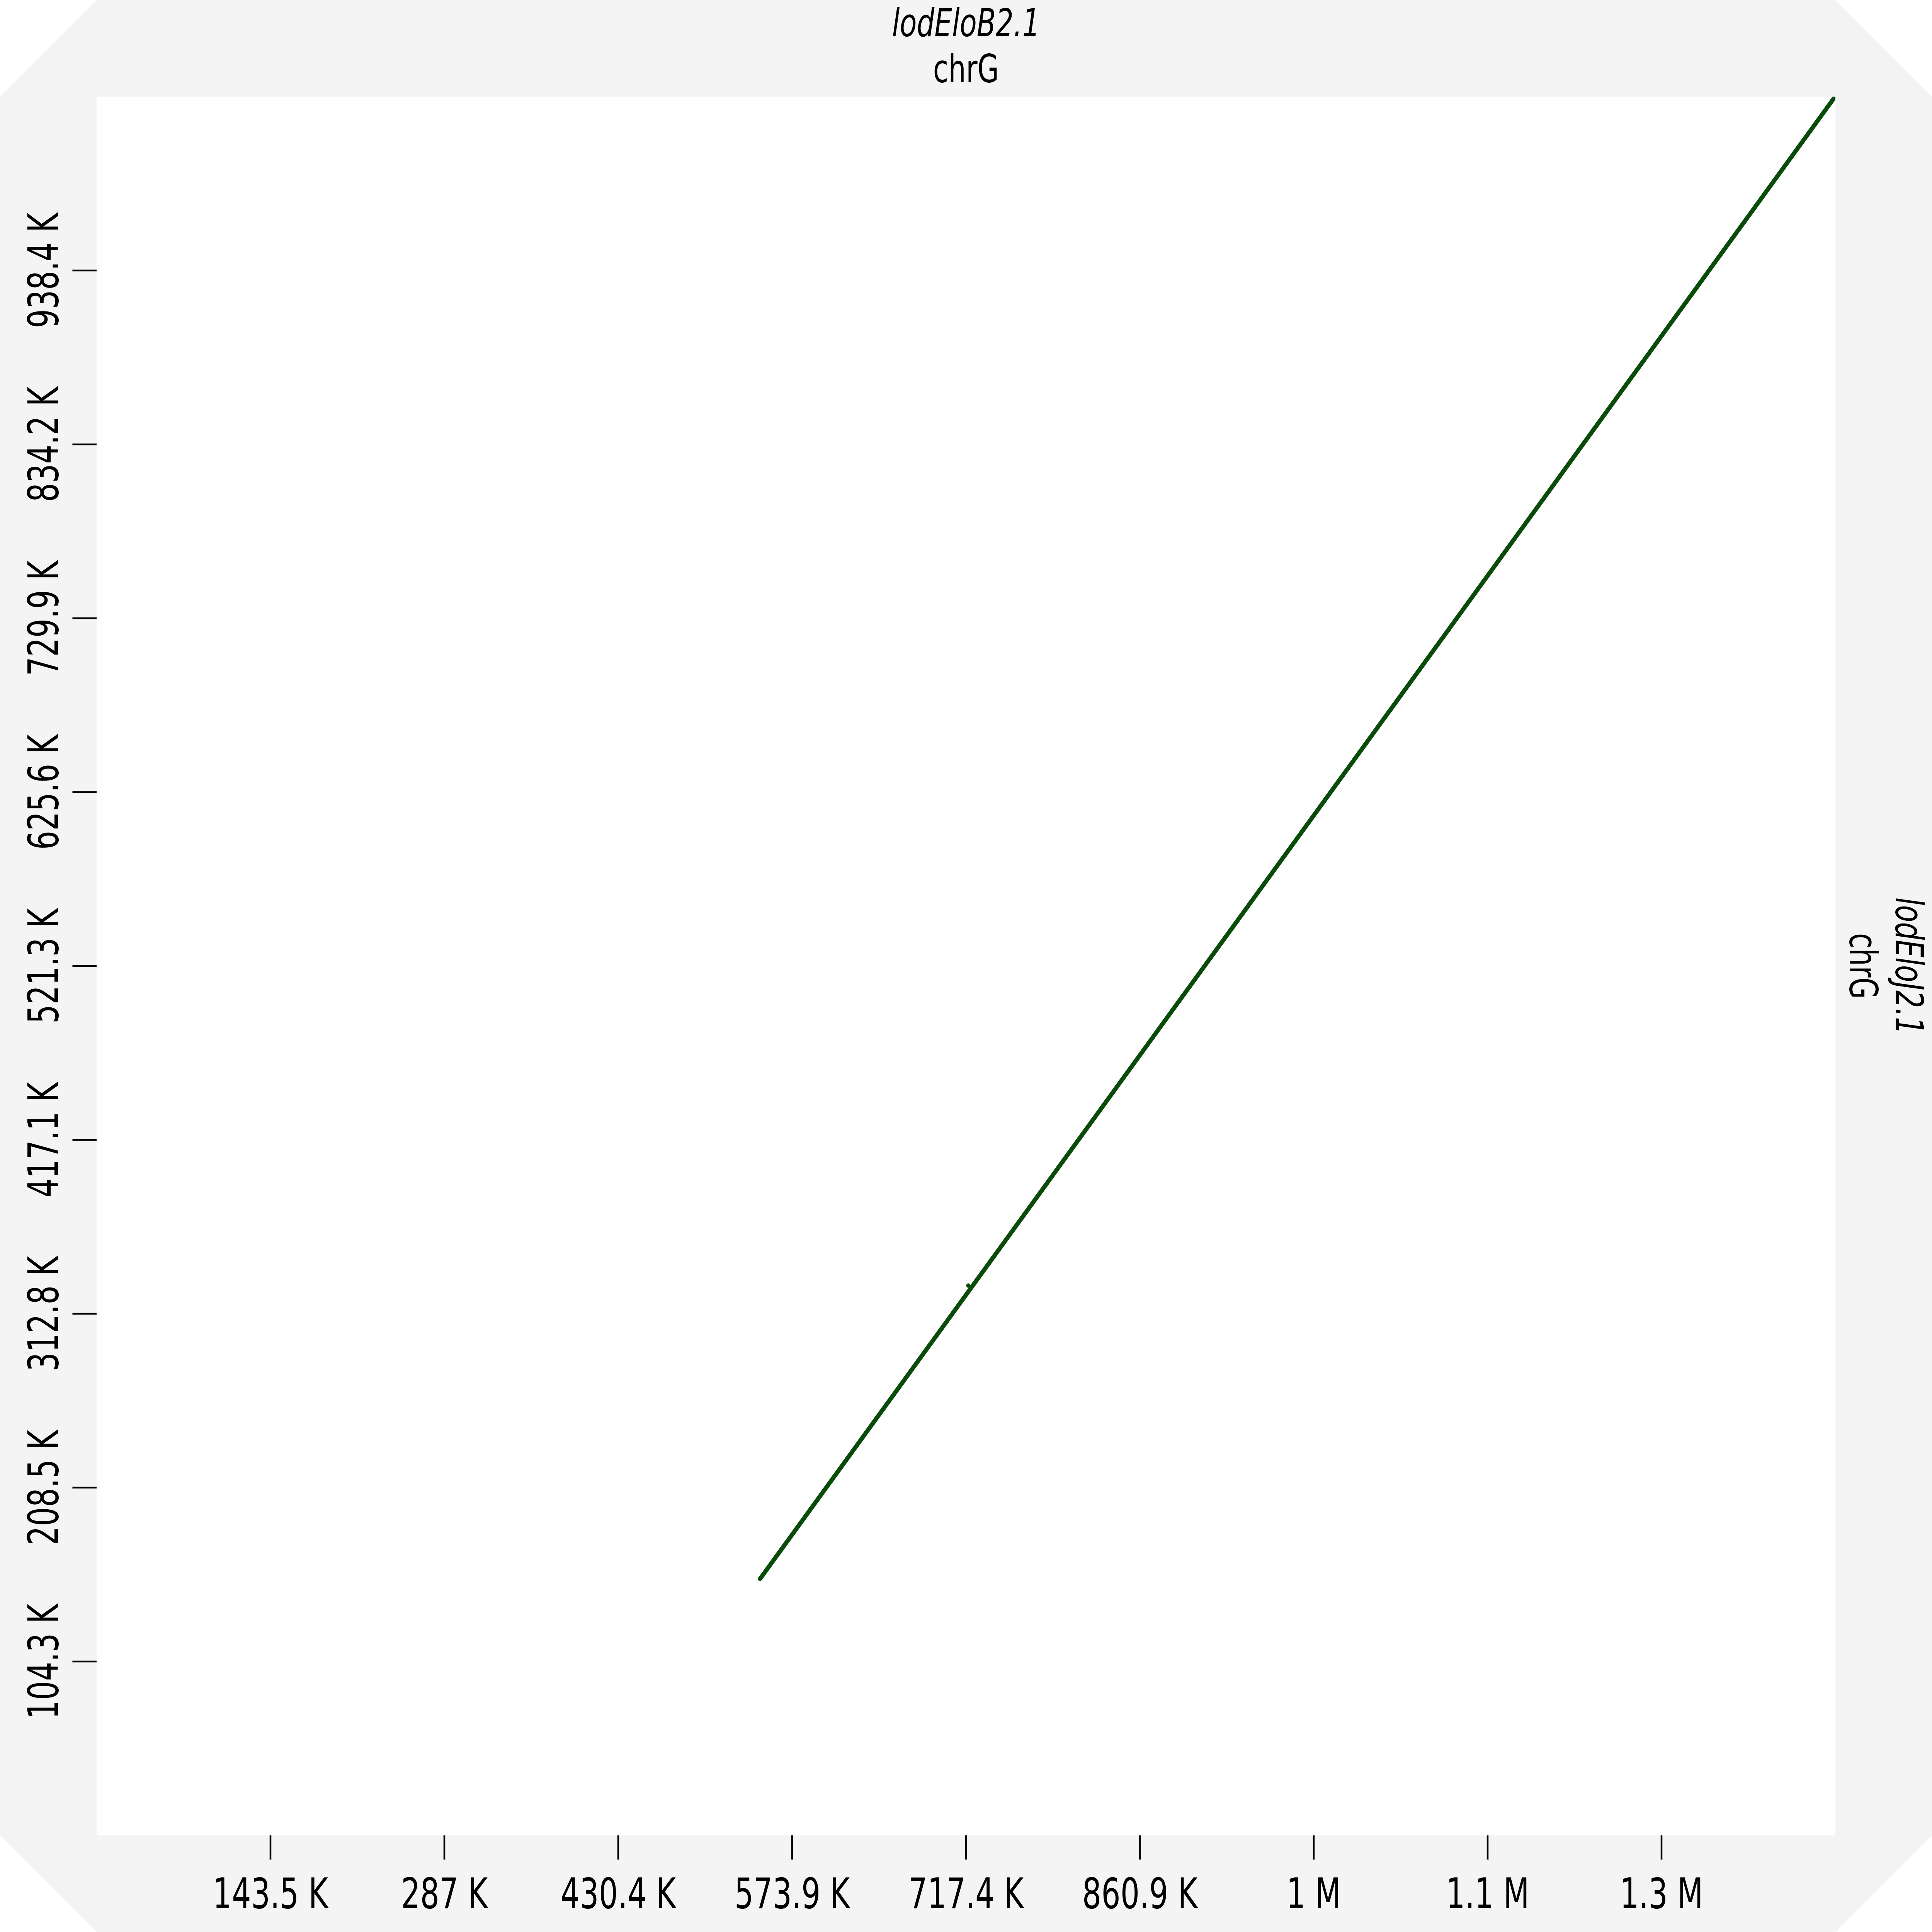
\includegraphics[width=.95\linewidth]{figures/lodelo/map_BG_JG.png}
%		\caption{Alignment between chromosome G of B2 and J2.}
%	\end{subfigure}%
%	\begin{subfigure}[b]{0.46\textwidth}
%		\centering
%		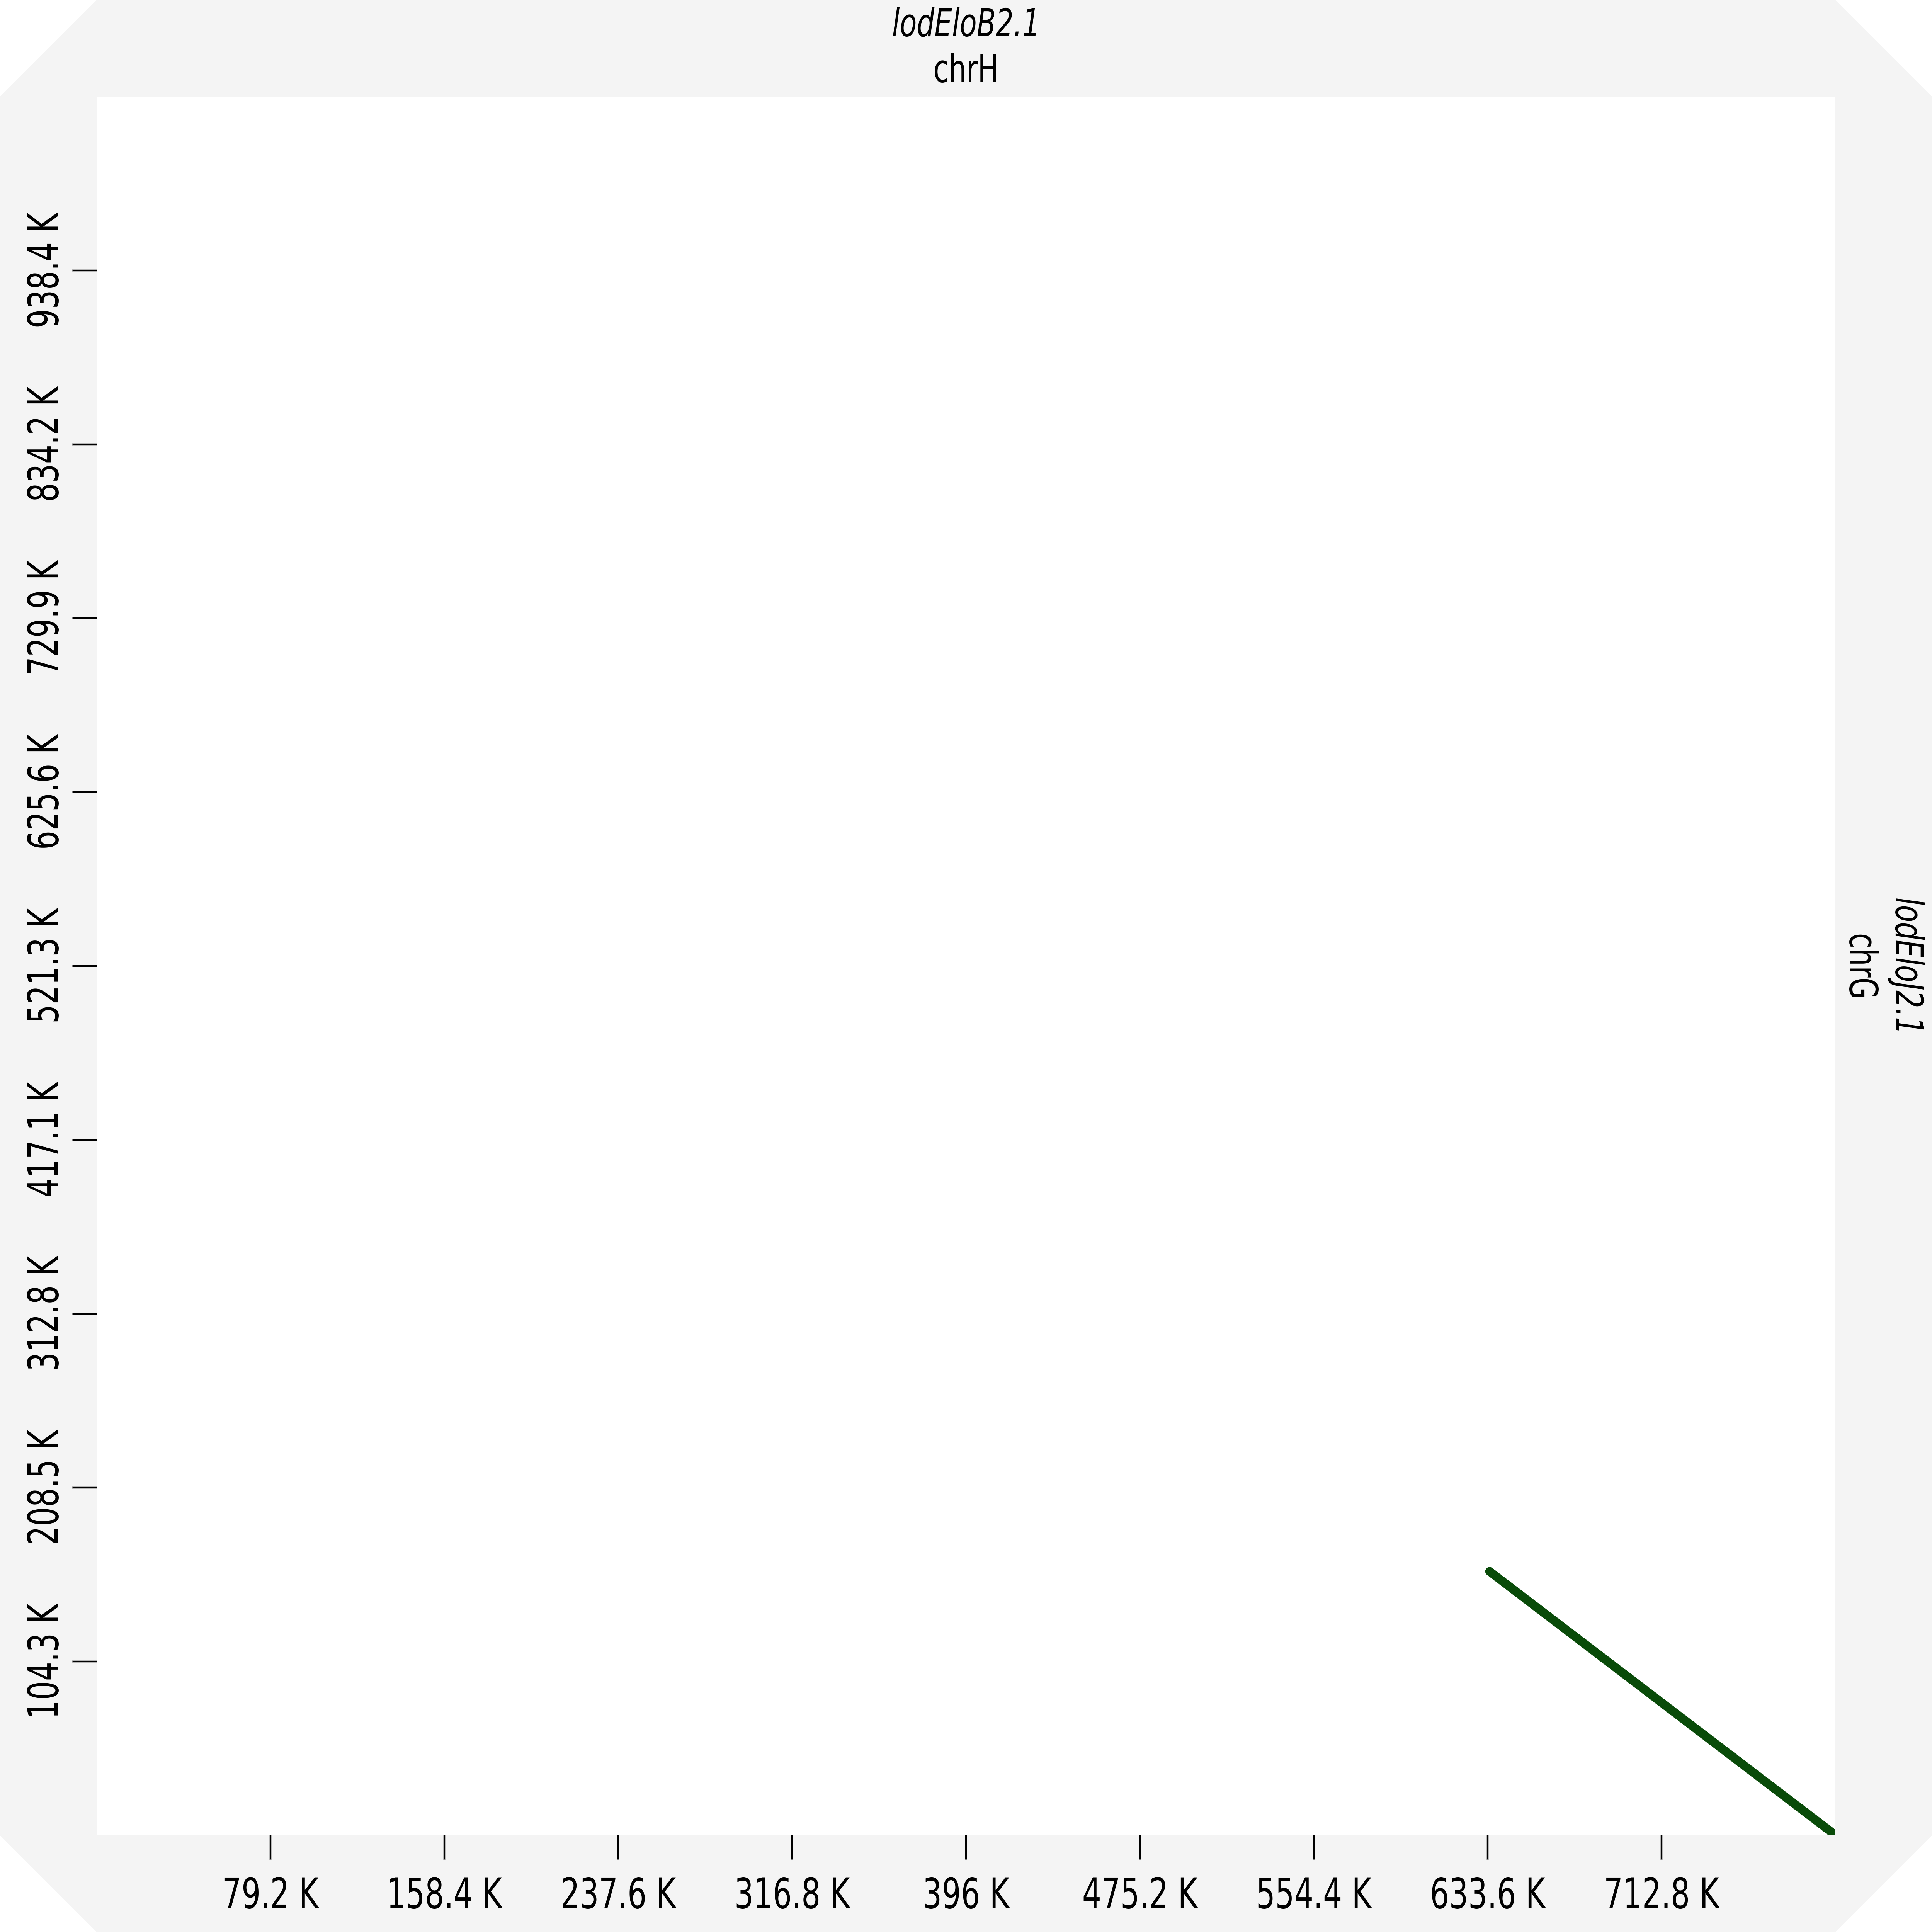
\includegraphics[width=.95\linewidth]{figures/lodelo/map_BH_JG.png}
%		\caption{Alignment between chromosome H of B2 and chromosome G J2.}
%	\end{subfigure}
%	\begin{subfigure}[b]{0.46\textwidth}
%		\centering
%		\caption{Alignment between chromosome C of B2 and J2.}
%	\end{subfigure}
%	\begin{subfigure}[b]{0.46\textwidth}
%		\centering
%		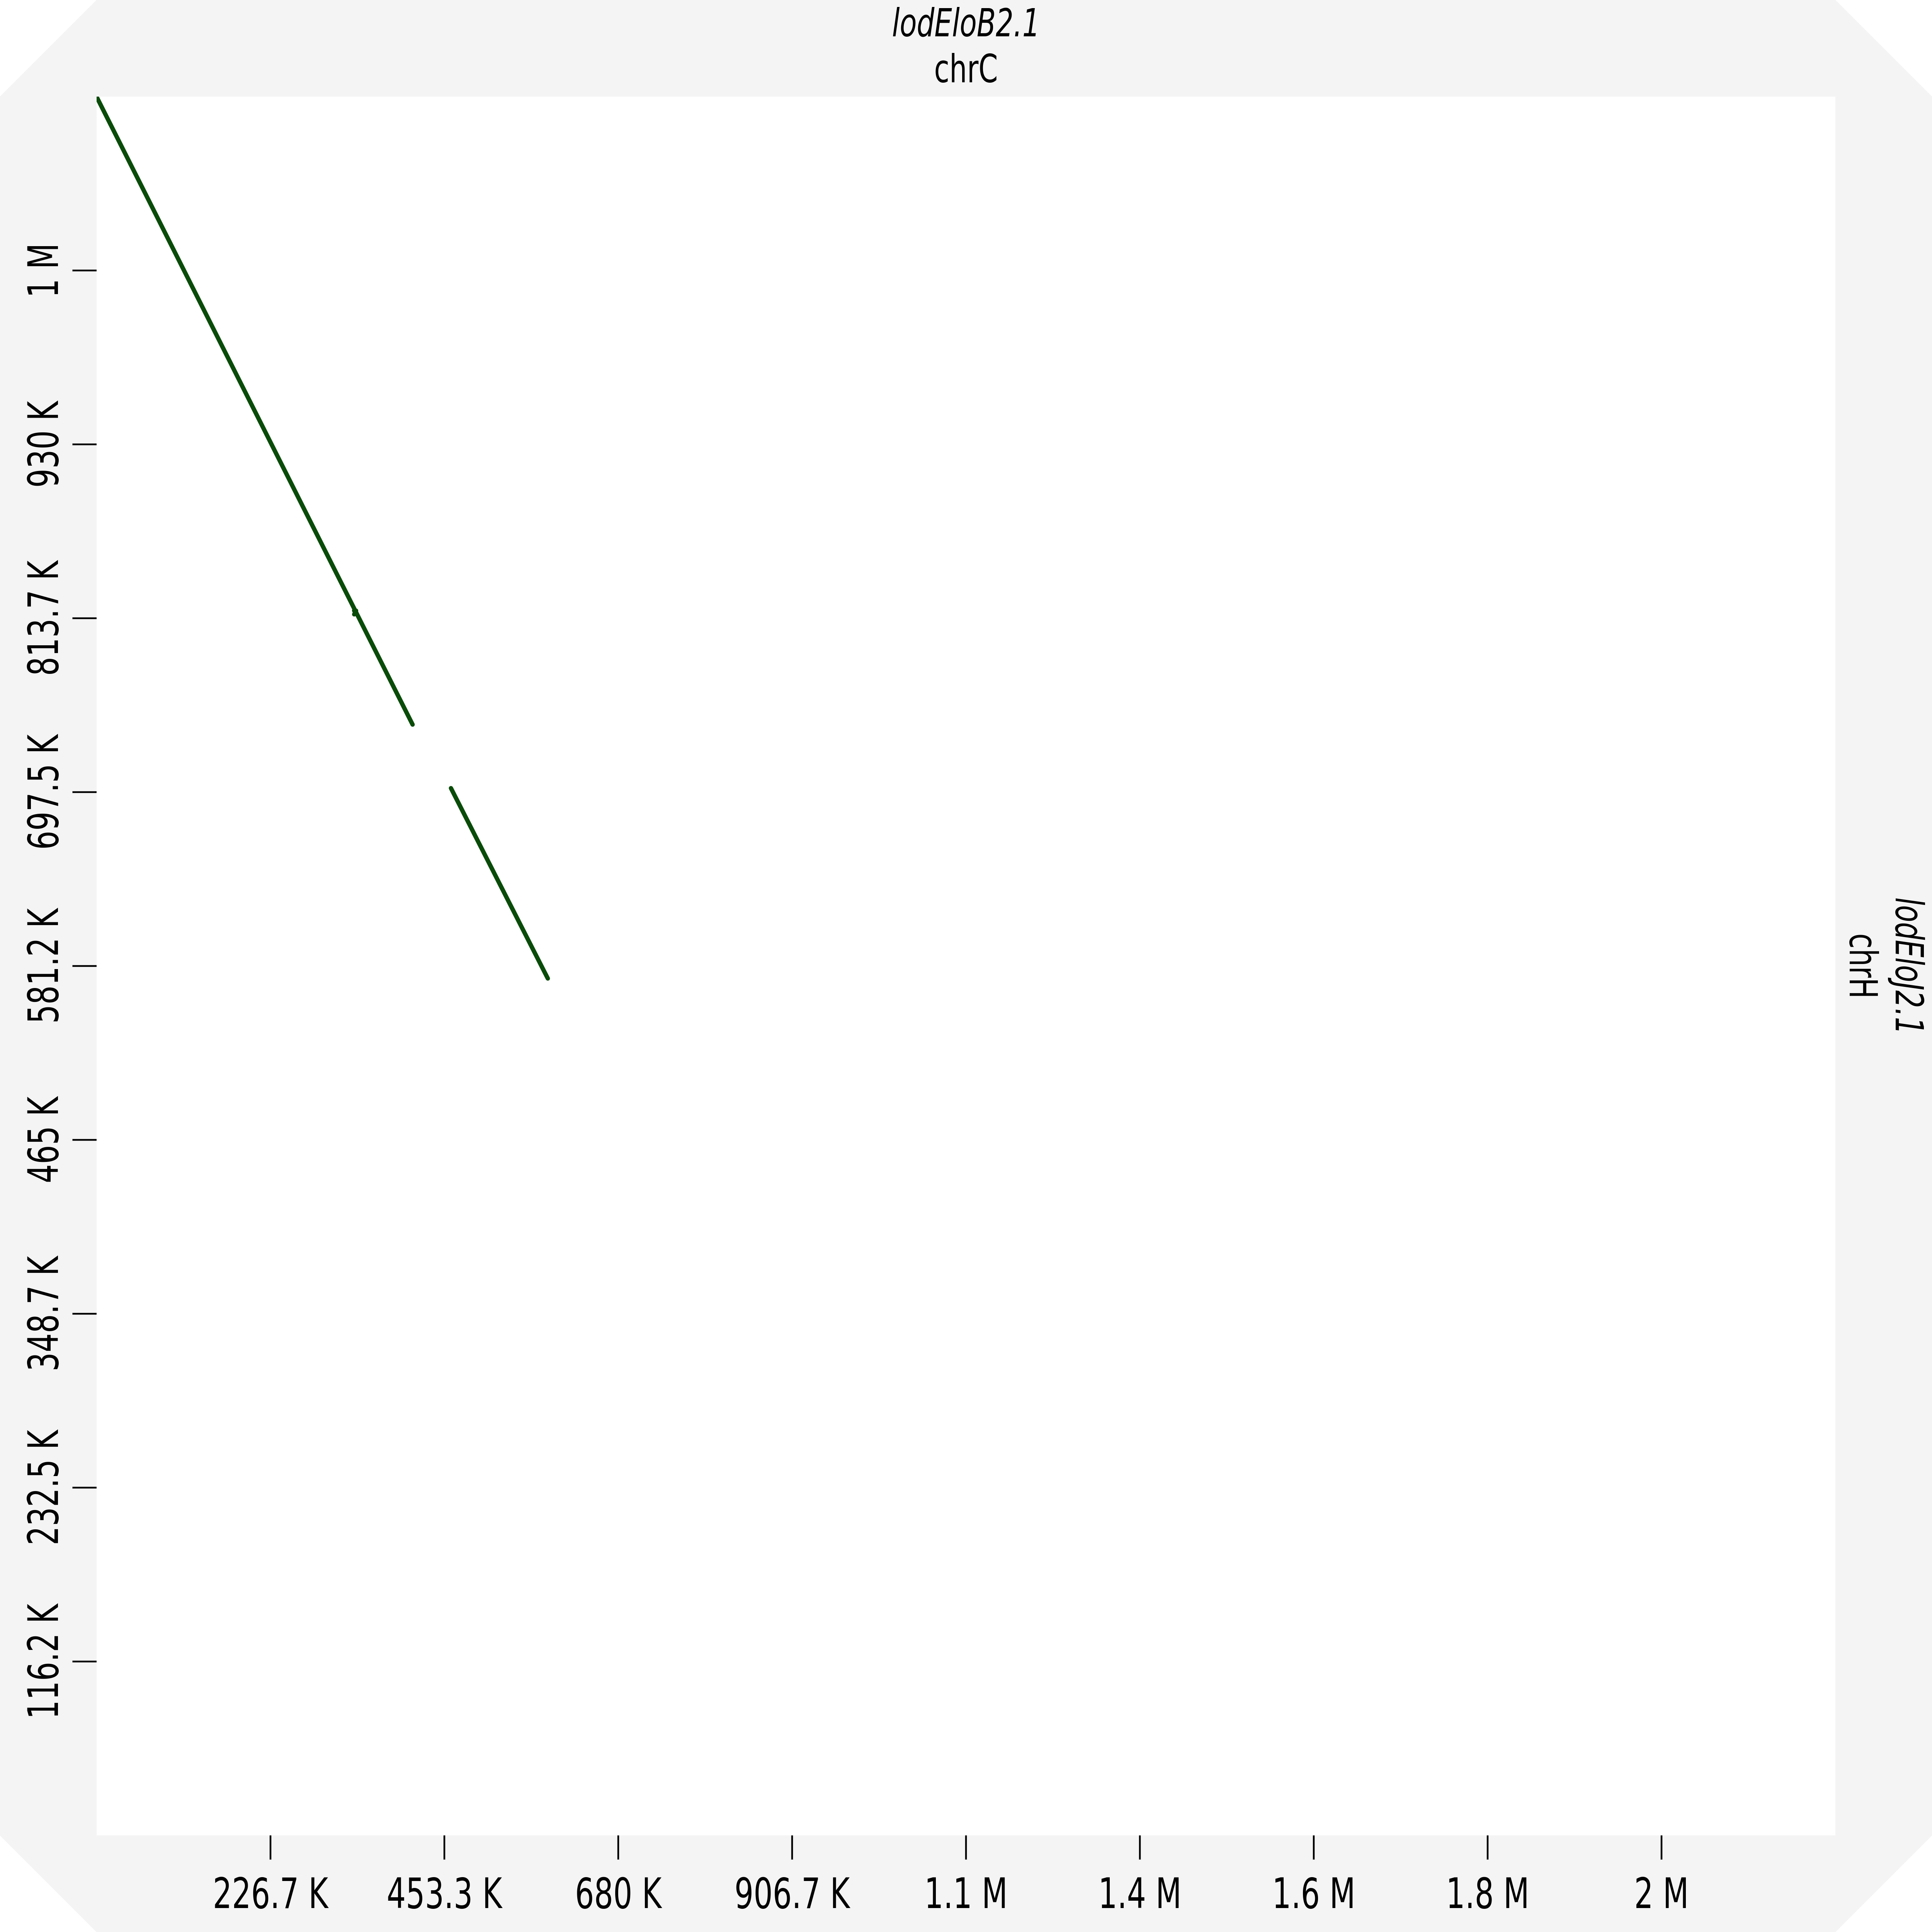
\includegraphics[width=.95\linewidth]{figures/lodelo/map_BC_JH.png}
%		\caption{Alignment between chromosome C of B2 and chromosome H of J2.}
%	\end{subfigure}
%	\caption{Dot-plot of the mapping of the resolved chromosomes of samples B2 and J2 for chromosomes C,G and H using D-Genies~\cite{dgenies} shows how large chunks of DNA is harbored into different chromosomes depending on the sample. Alignments were obtained using \wfmash \texttt{-p90 -s10000}.}
%	\label{fig:lodelo_dotplot-alignments}
%\end{figure}

%The consortium my phd fellowship belongs to, the EU Commission founded Marie Curie ITN Alpaca (Algorithms for Pangenomic computational analysis) consortium~\cite{alpacawebsite}, organized a winter wet-lab school to give a small training on how the processing of preparing samples for sequencing works, in order to improve the knowledge on the full stack of processes done to obtain genomes from biological samples of the medically interesting yeast strain of \lodelo. From 11 different samples, we generated long (ONT) reads, in collaboration with a lab at the Comenius University in Bratislava, Slovakia. We divided into several groups to perform different genomic analyses on it. One of these team, the one I was in, was tasked on building a pangenome reference of \lodelo. \\ 
%We sequenced,  The computational work I present here was done in collaboration with members of the consortium, in large part by Simon Heumos, whom I would like to thank for the time spent discussing and working together.

\subsection{\emph{Lodderomyces elongisporus}: genetic characteristichs, interest and used data}
\emph{Lodderomyces elongisporus} is a diploid yeast that has been isolated from, among many sources, humans and it is recently emerging as pathogenic. It is phylogenetically placed in the Candida clade and the size of its genome is usually between 15 and 16 Mb, 2 orders of magnitude smaller than a human genome~\cite{Lodderomyces}. Its DNA is organized into 8 chromosomes, that here will be referred in alphabetical order and decreasing size A to H, from around 3.5Mbp of chr A to 800 Kbp of chr H, plus a 35 Kbp mitochondrial DNA. Our analysis shows that it has a stable core genome of ~13Mbp, as shown in section~\ref{sec:core_pg}. 
Increasing reports of (mostly bloodstream) infection in mainly immunosuppressed adults makes it an increasingly important subject of studies\cite{lodelo_pathogen,lodelo_fatal,lodelo_meningitis,lodelo_bloodstream}: it also got recent attention when an outbreak was reported occurring in a neonatal ICU in Dheli, India from September 2021 to February 2022 with 1 death\cite{lodelo_india}.\\
Samples sequenced by us were called in alphabetical order, followed with a number greater or equal than 0 that denoted the quality of the assembly. Moreover, one sample, B2, for which a member of the consortium produced a high quality assembly after manual curation, was used as relative reference in the cohort. Another sample, J2, was also fully resolved into chromosomes while the others were assembled into contigs.

\begin{table}
	\centering
	\begin{tabular}{| c | c | c | c | c | c | c | c | c | c | c | c | c | c |}
		\hline
		filename     &   total length   & number of sequences & mean length &    longest & shortest     &   N count & Gaps &   N50  &   N50n  &  N70 &    N70n &   N90 &    N90n \\
		\hline
		A1 & 15699113 & 25 & 627964.52 & 2595744 & 3907 & 0 & 0 & 1354781 & 5 & 938474 & 8 & 414196 & 13 \\
		B2 & 15485469 & 7 &  2212209.86 & 4493495 & 35166 & 0 & 0 & 3516991 & 2 & 2001278 & 4 & 1643619 & 5 \\
		C0 & 15532065 & 20 & 776603.25 & 3532941 & 810 & 0 & 0 & 1331232 & 4 & 1222310 & 6 & 835847 & 9 \\
		D0 & 15507665 & 17 & 912215.59 & 3532853 & 5008 & 0 & 0 & 2160581 & 3 & 1885061 & 5 & 740828 & 7 \\
		E0 & 15332588 & 18 & 851810.44 & 3544471 & 3228 & 0 & 0 & 1992182 & 3 & 1040518 & 6 & 418294 & 10 \\
		F1 & 15664073 & 21 & 745908.24 & 3548518 & 1282 & 0 & 0 & 2165076 & 3 & 1245669 & 5 & 440649 & 9 \\
		G0 & 15636520 & 19 & 822974.74 & 3548910 & 550 & 0 & 0 & 1697956 & 4 & 1657398 & 5 & 527890 & 9 \\
		H0 & 15601346 & 21 & 742921.24 & 3549008 & 6842 & 0 & 0 & 2170489 & 3 & 1247137 & 5 & 469363 & 10 \\
		I1 & 15639882 & 30 & 521329.40 & 3622524 & 536 & 0 & 0 & 1999295 & 3 & 1636379 & 5 & 384387 & 10 \\
		J2 & 15425942 & 9 & 1713993.56 & 3543738 & 35442 & 0 & 0 & 2157297 & 3 & 1647795 & 5 & 1162477 & 7 \\
		K0 & 15752744 & 16 & 984546.50 & 3534745 & 19835 & 0 & 0 & 1631500 & 4 & 1305577 & 6 & 684340 & 9 \\
		\hline
	\end{tabular}
\end{table}

\subsection{Building ad hoc pangenome reference}
We produced a \dbg of the assemblies using \bifrost, but their usefulness remains limited for visual analysis of complex biological events interpretation and study.\\
Figure~\ref{fig:lodelo_dbg} shows the visualization of the \dbg for \kmer length equal to 25: redundant parts of the genome make the graph collapse. This is the same phenomenon previously described for human genomes, as better insight can be acquired when just a small region is visualized. 
De Bruijn Graphs can instead be useful for to produce quite straightforward whole-genome alignment- and reference-free phylogenetic analysis in a fraction of time required by competitor methods that use all vs. all alignment. The tool \sans~\cite{sans} can process directly a \bifrost generated \ccdbg to estimate the phylogenetic splits between the genomes contained in the graph. Figure~\ref{fig:dbg_phyl} shows the visualization of the phylogenetic network produced by \sans using the tool \splitstree~\cite{splitstree}. This results shows how \dbgs are quite powerful when applied to specific applications.\\
\begin{figure}[h!]
	\centering
	\begin{subfigure}[b]{0.75\textwidth}
		\centering
		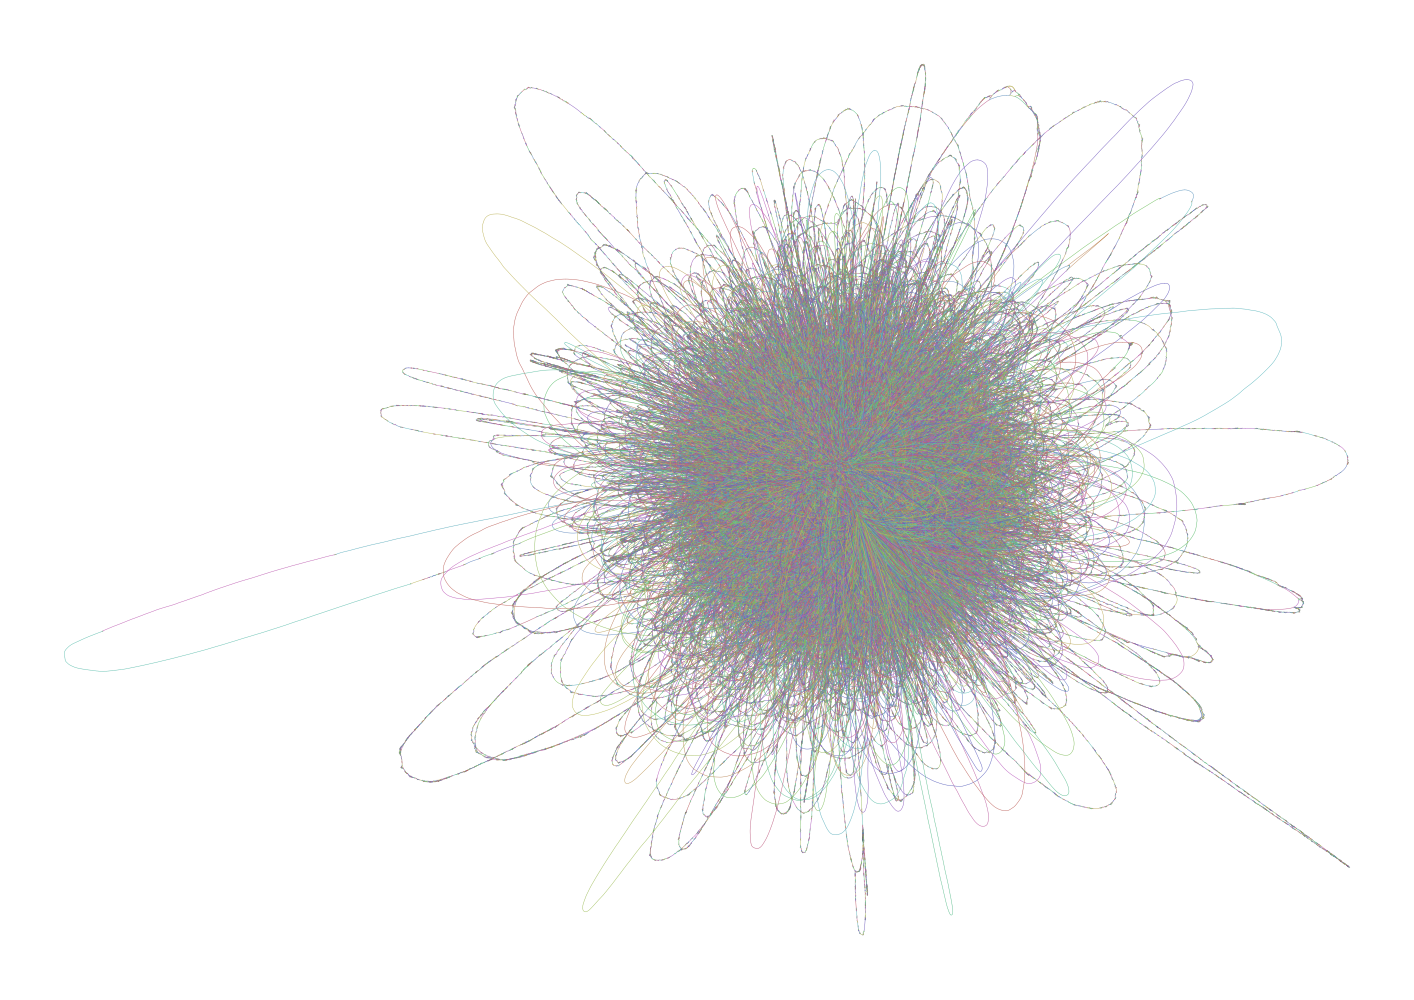
\includegraphics[width=1\linewidth]{figures/lodelo/lodElo_k25.png}
		\caption{\bandage visualization of the pangenome \dbg of the cohort of 11 \lodelo strains. As for human genomes, visualization of the whole data offers no particular insight, apart from the large variations visible on the rounded parts away from the dense part.}
		\label{fig:lodelo_dbg}
	\end{subfigure}%
	\\
	\begin{subfigure}[b]{0.75\textwidth}
		\centering
		\includegraphics[width=1\linewidth]{figures/lodelo/direct_nobei.png}
		\caption{\splitstree visualization of the phylogeny network generated using \sans from the \ccdbg constructed using \bifrost.}
		\label{fig:dbg_phyl}
	\end{subfigure}%
	\caption[\ccdbg representation and phylogeny analysis of the \lodelo pangenome.]{Visualization of the \ccdbg representation and phylogeny analysis of the \lodelo pangenome.}
\end{figure}
Given high quality assemblies generated by the sequences of these 11 samples, we decided to also build a pangenome graph with small variant resolution using \pggb and \mcactus, in a similar way to what has been done with the Human Draft Pangenome Reference~\cite{hdpr}. It is important to notice that in order to produce the best biological correct result, several rounds of parameter tuning and manual curation are needed, with knowledge far superior of the one of a first-time user.\\
The first step to build such pangenomes is to divide the genome assemblies into communities of sequences belonging to chromosomes.

%As explained before, variation graphs generation is given by communities separation. \pggb works by building a single graph from a given community, so it fits well for this specific use-case: by grouping together the contigs corresponding to the three chromosomes where the recombination occurred, the pipeline should produce a graph that consider this event.
\subsubsection{Determining chromosomal communities}
Variation graphs construction pipelines use mapping or alignment between the input set of genomes to infer graphs. Their first step consists in grouping the sequences from the assemblies into communities representing a chromosome in order to run a single computation instance and produce a separate graph for each of them. The final graph is then given by joining together the output of each group. This means that without any pre-processing, no inter-chromosomal event can be detected.\\ 
In this specific use-case, in order to identify inter-chromosomal events, contigs associated to any of the 3 chromosomes conjectured to be part of the rearrangement had to fall into the same community and be provided together in input to the pipeline. This would ensure that, if such rearrangement exists, it would produce a feature in the graph that would show as a tangle between the chromosomes.\\
As the rest of the assemblies, with the exception of the J2 sample, were not resolved into single chromosomes, each of them was aligned to the reference B2 using \wfmash alignment segment size of 10k and 95\% sequence identity (and lower segment size, 90\% sequence identity if unmapped). The identity scores of the alignment of the genomes to the reference B2 assembly is shown in figure~\ref{fig:lodelo_alignment_scores}. From this alignment, contigs were assigned to the chromosomal community to which they best mapped. Finally, the ones of chromosome C, G and H were grouped into a single one.
\begin{figure}[h!]
	\centering
	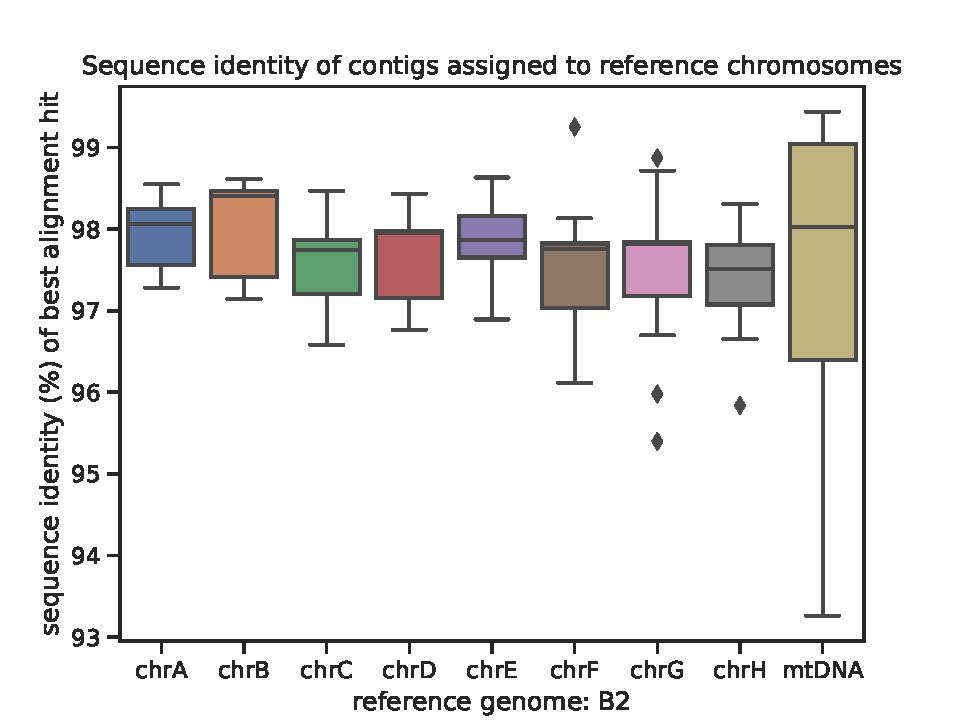
\includegraphics[width=.8\linewidth]{figures/lodelo/Alignment_scores.pdf}
	\caption[Sequence Identity of \lodelo samples's contigs assigned to reference chromosomes.]{Sequence Identity of contigs assigned to reference chromosomes. Image produced using a pipeline developed by Simon Heumos.}
	\label{fig:lodelo_alignment_scores}
\end{figure}

\subsubsection{Producing a variation graph using pggb}
As \pggb uses all-vs-all alignment of a collection of sequence as first step to infer the graph, it enables the representation of recombination among chromosomes placed inside the same community, as seen also for human acrocentric chromosomes~\cite{Guarracino2023}.\\
By simply running the \texttt{nextflow/pangenome} (\pggb) pipeline, we were able to produce a first pangenome representation of the 11 yeast strains. The tangle visible in figure~\ref{fig:lodelo_gfaestus} clearly shows the recombination happening between the three chromosomes. This work was mainly done by Simon Heumos and the graph shown in figure ~\ref{fig:lodelo_gfaestus} is the result of more than 25 rounds of parameters tuning.
The detection of the event with a variation graph using \pggb encouraged the effort to produce a similar representation with \mcactus, a pipeline that is not designed to construct grouped chromosomes pangenomes.
\begin{figure}[h!]
	\centering
	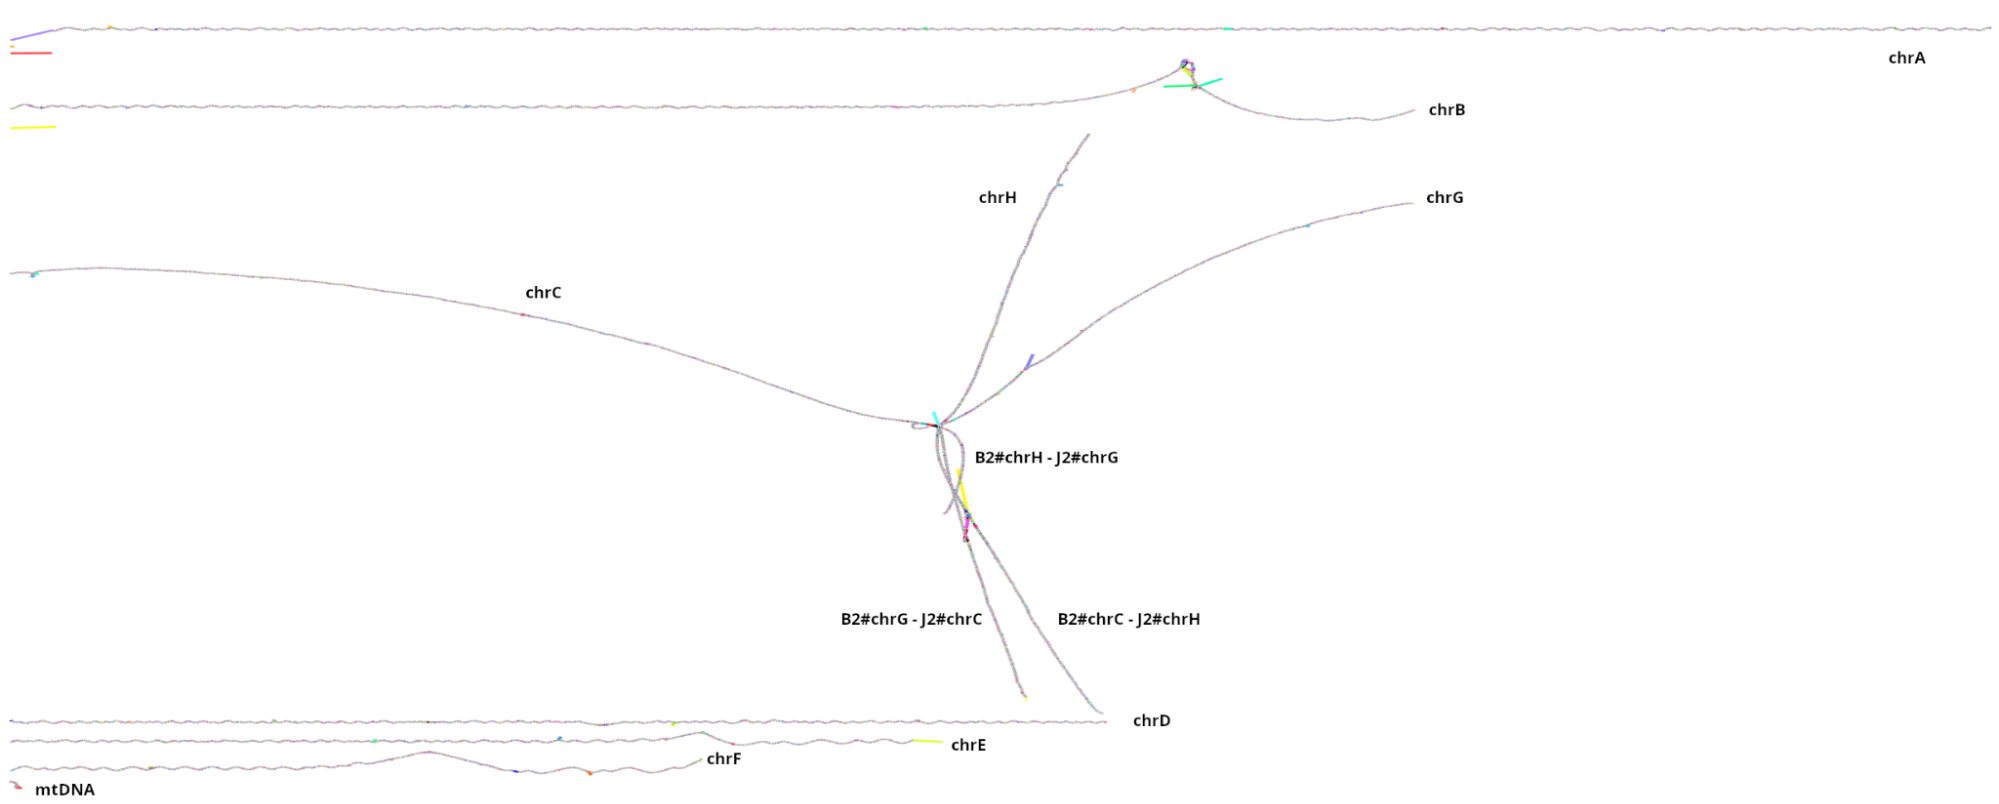
\includegraphics[width=.8\linewidth]{figures/lodelo/pggb_full.png}
	\caption[\gfaestus visualization of a \lodelo variation graph.]{\gfaestus visualization of the \pggb variation graph of the 11 \lodelo samples. Image produced by Simon Heumos.}
	\label{fig:lodelo_gfaestus}
\end{figure}


\subsubsection{Overcoming \mcactus limitation by modifying both the data and the pipeline}
In order to produce a graph that represents variation between multiple chromosome with \mcactus, a custom pipeline has to be used. \mcactus communities are implicitly inferred by the first step, performed by \minigraph. For this tool, the chromosomes present in the first reference genome given as input are used as communities and backbone for the whole graph and no sequence can be both assigned to different chromosome. This is an intrinsic characteristic of \minigraph and cannot be changed with input parameters: it means that there is no feature to have chromosome C,G and H considered together in input.\\
To try to overcome this limitation of the approach we tried to produce a graph that respected the condition of having the three chromosome inside the same connected component, at the cost of producing a representation that was not biologically correct. We therefore produced a chimeric contig consisting of the concatenation of the three chromosomes assemblies of the B2 sample. The rationale was to provide the 3 chromosomes chained together as a single backbone in the \minigraph construction step. This would allow sequences to be mapped to any of chr C, G and H to be considered together in the subsequent steps of alignment and graph the \mcactus pipeline. The expectation was to therefore produce a graph that showed the recombination from the mapping of the contigs of the other genomes. \\
By building a graph using \minigraph with the chimeric chromosome CGH and all the contigs of the other genomes assigned to chromsome C, G and H does not represent any recombination event, as can be seen in figure~\ref{fig:cgh_mingraph}. This was somewhat expected, as it is known that \minigraph does not also consider inversion between genomes.
When the complete modified pipeline of \mcactus is run, it is possible to see the tangle between the chromosomes, as shown in figures~\ref{fig:cgh_mcactus}~\ref{fig:lodelo_graph_tangle}.
\begin{figure}[h!]
	\centering
	\begin{subfigure}[b]{\textwidth}
		\centering
		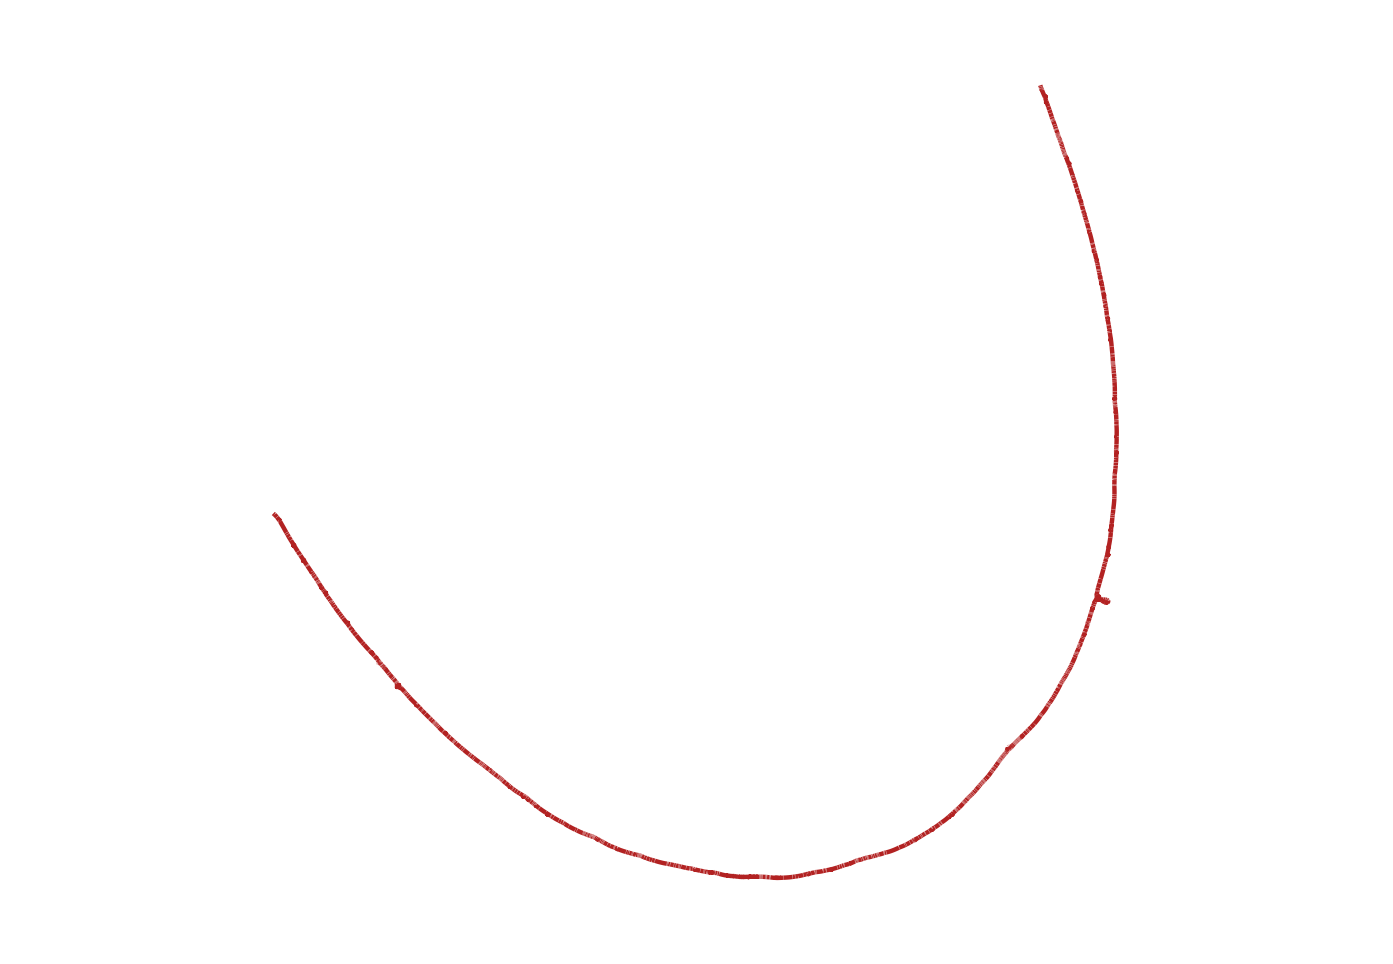
\includegraphics[width=.4\linewidth]{figures/lodelo/minigraph_cgh.png}
		\caption{Graph of chimeric chromosome CGH from sample B2 and all the contigs of the other genomes aligning to it produced with \minigraph. The graph is linear and no inter-chromosomal event is visible.}
		\label{fig:cgh_mingraph}
	\end{subfigure}%

	\begin{subfigure}[b]{\textwidth}
		\centering
		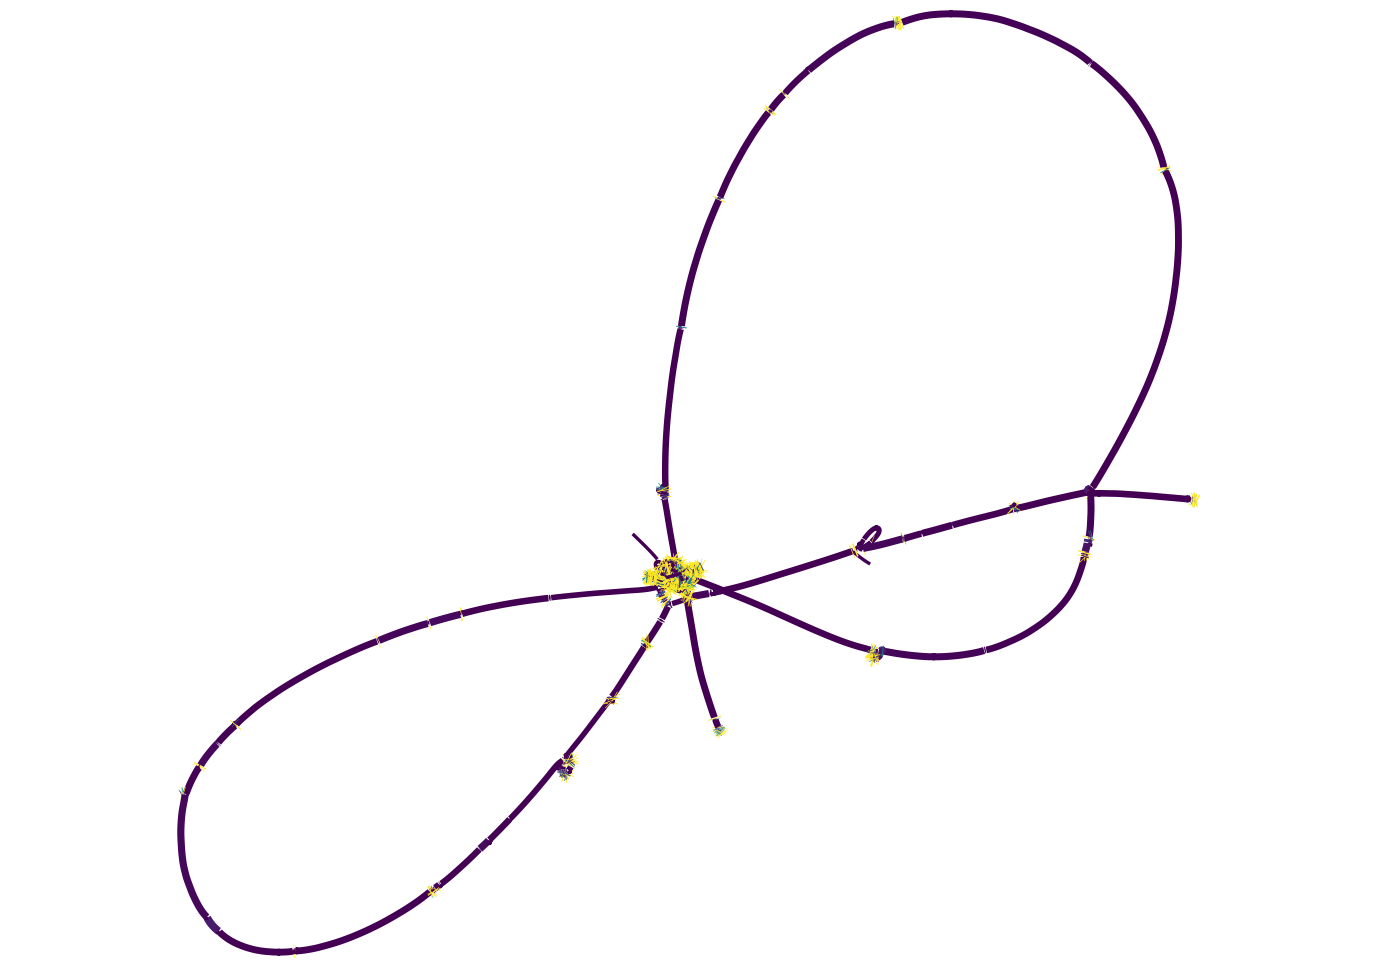
\includegraphics[width=.4\linewidth]{figures/lodelo/mcactus_cgh_u1000_by_depth.png}
		\caption{The graph after all the other steps of the \mcactus pipeline, colored by depth, after simplification of variants < 1kbp using the command \gfatools  \texttt{asm -b 1000 -u}. The large recombination event is now visible.}
		\label{fig:cgh_mcactus}
	\end{subfigure}
	\caption[Difference in output between \minigraph and \mcactus.]{Difference in output between \minigraph and \mcactus of the chimeric graph produced to visualize the inter-chromosomal event between C,G and H.}
	\label{fig:chromosome_cgh_minigraph}
\end{figure}

\subsection{Representing translocation events from groups of genomes}
Applying simple community separation on the all vs all alignment of the contigs, like the one suggested in the manual of \pggb, does not help confirming the hypothesis, mainly because of segment length selection. Figure~\ref{fig:lodelo_communities} shows community detection using Louvain algorithm on the contig network inferred by all vs all alignment.
\begin{figure}[h!]
	\centering
	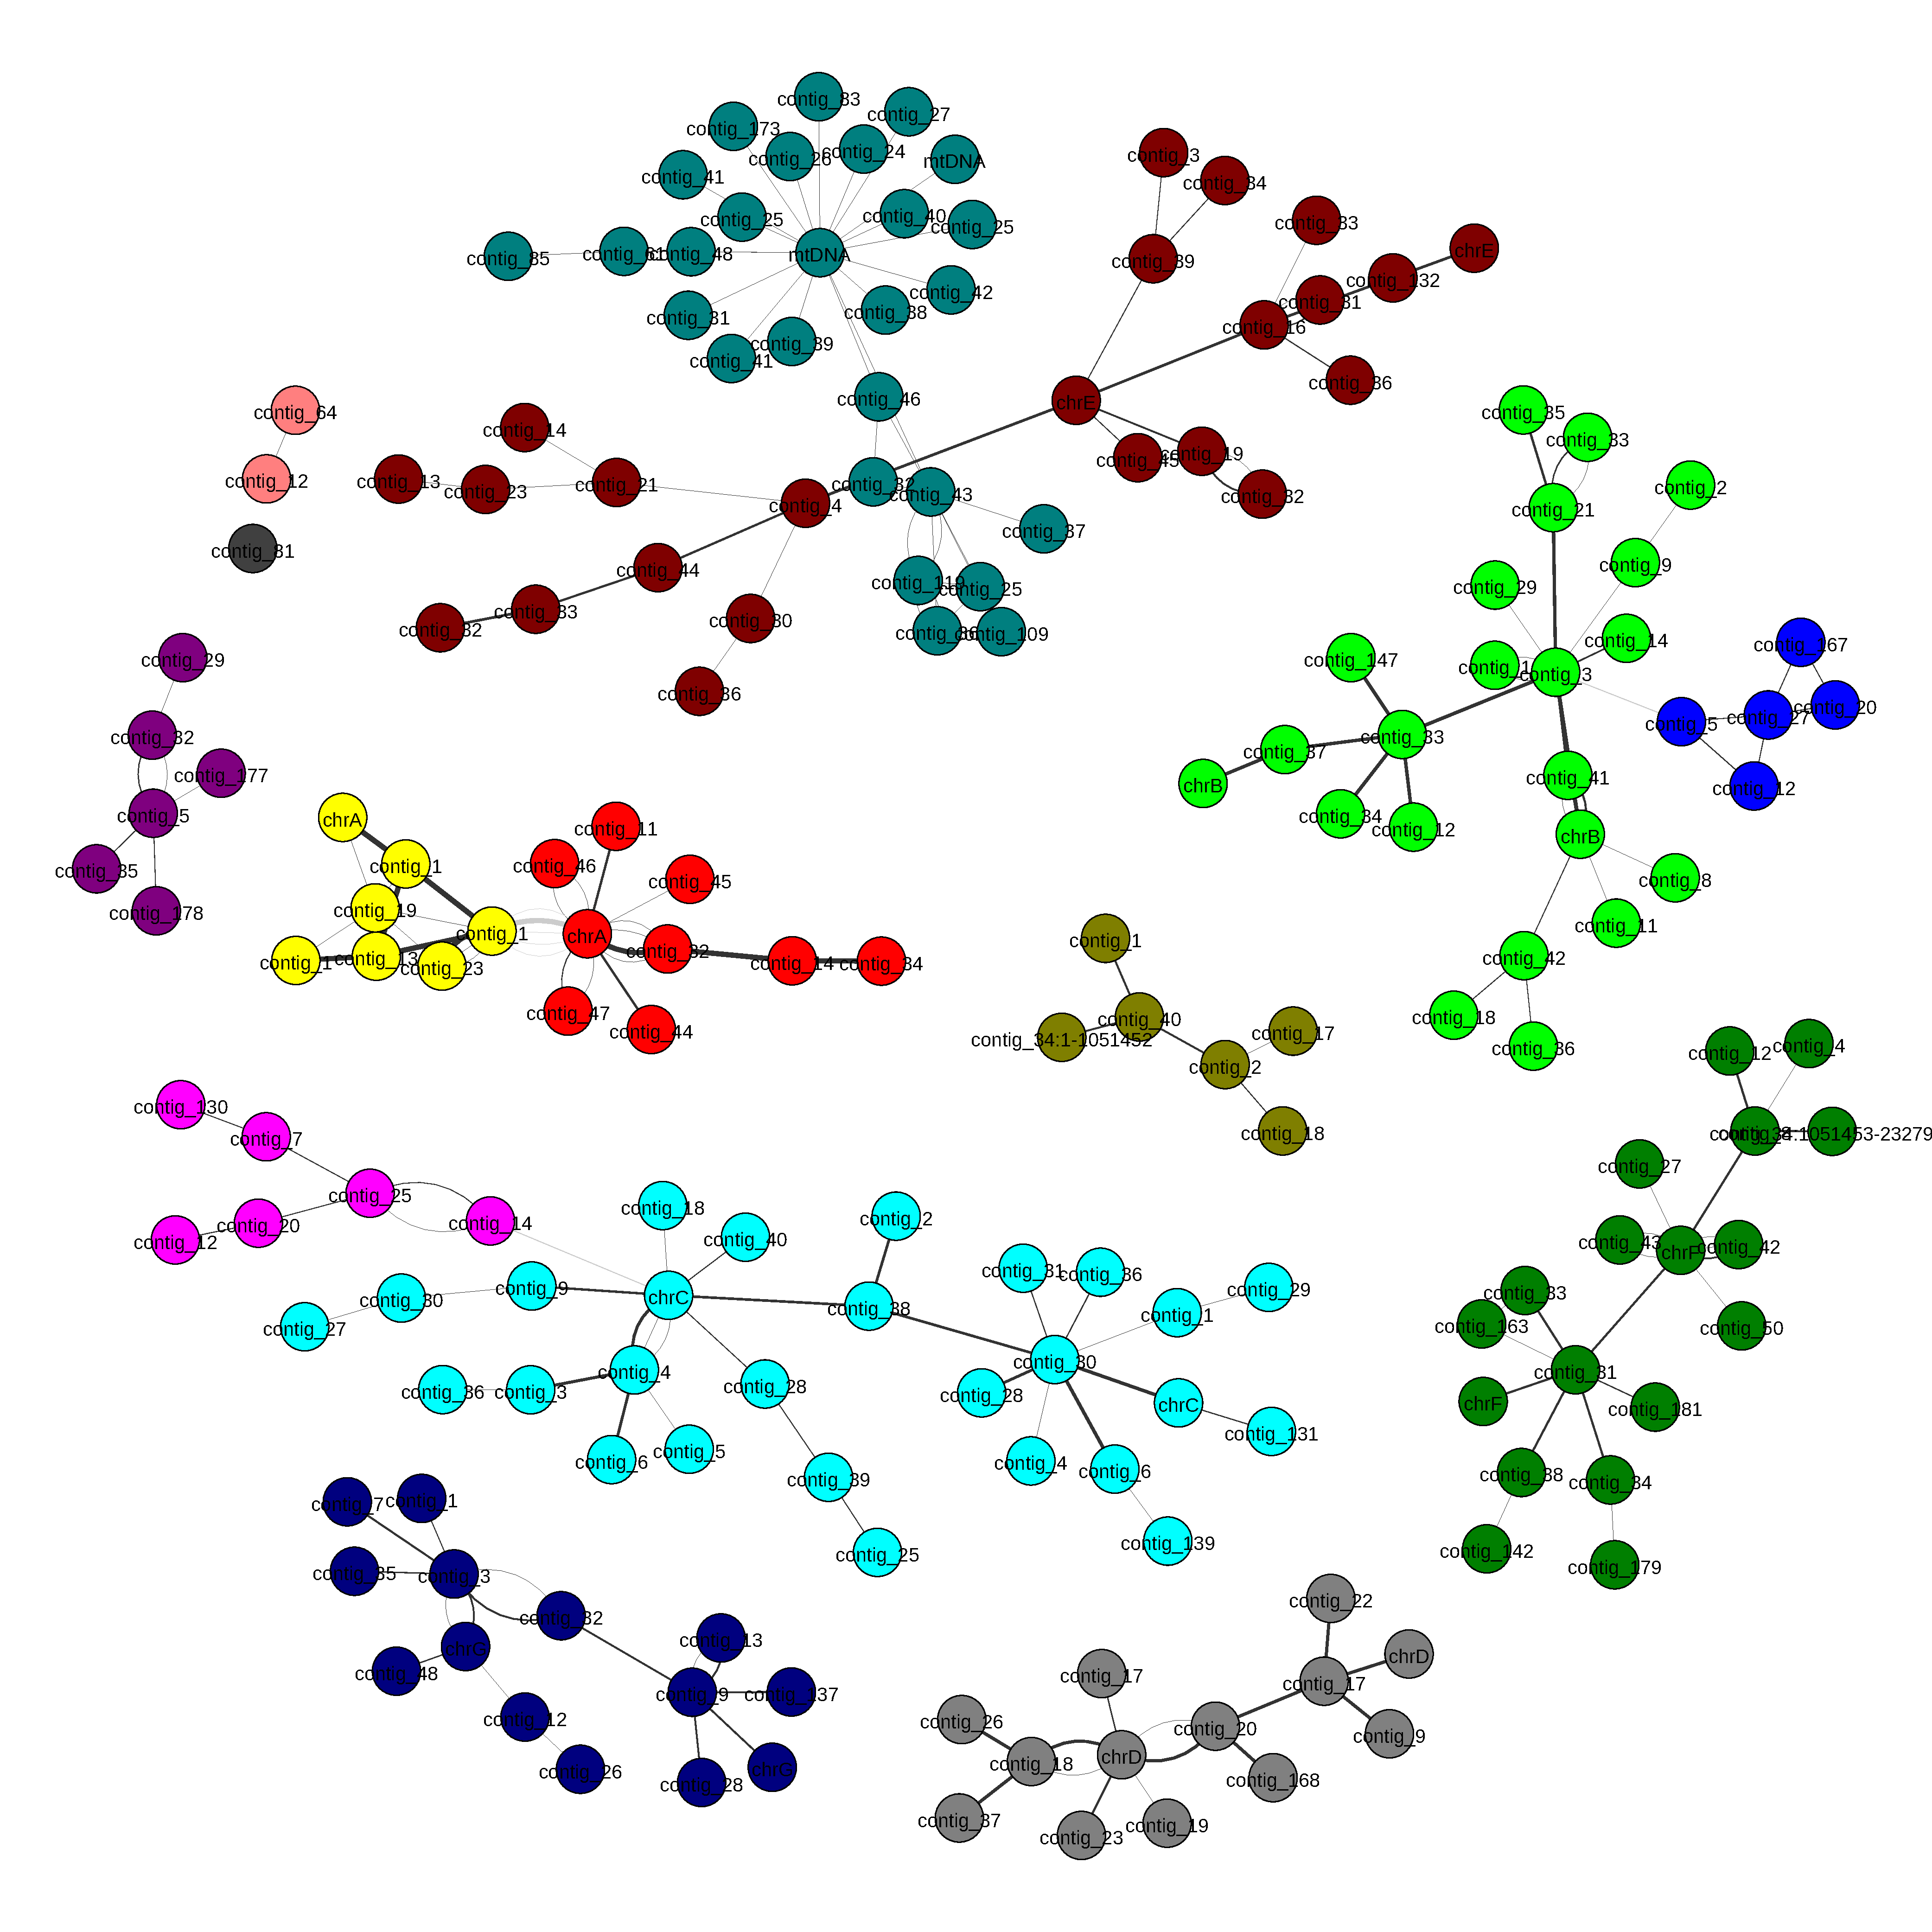
\includegraphics[width=.4\linewidth]{figures/lodelo/alingment_communities.pdf}
	\caption[Community partition of the contigs to detect inter-chromosome events.]{Community partition of the contigs based on all-vs-all alignment scores.}
	\label{fig:lodelo_communities}
\end{figure}
This inter-chromosomal rearrangement is instead detectable using linear whole-genome assembly based tools. By aligning J2 to the relative reference genomes B2 with \wfmash and then looking for syntenies and rearrangements with \syri, it is possible to detect syntenic path (longest set of co-linear regions), structural rearrangements (inversions, translocations, and duplications)~\cite{syri}. Figure~\ref{fig:plotsr_synteny} shows the detected rearrangements and duplications between the 3 chromosomes using \plotsr~\cite{plotsr}.
While figure~\ref{fig:plotsr_synteny} shows in a clear way the kind of inter-chromosomal variation between the 2 strains, \syri does work only with genomes resolved to chromosome level. This means that such analysis is not possible on the whole cohort using standard linear reference tools. 
\begin{figure}[h!]
	\centering
	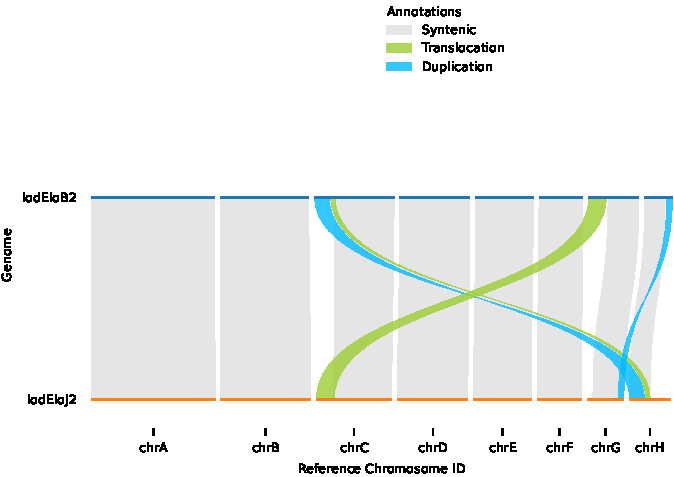
\includegraphics[width=.8\linewidth]{figures/lodelo/plotsr.pdf}
	\caption[Linear reference visualization of the \lodelo inter-chromosomal recombination.]{\plotsr visualization of the inter-chromosomal recombination detected using \wfmash and \syri.}
	\label{fig:plotsr_synteny}
\end{figure}
It is therefore possible to visualize the tangle that emerges from the graph generated with \mcactus. 
\begin{figure}[h!]
	\centering
	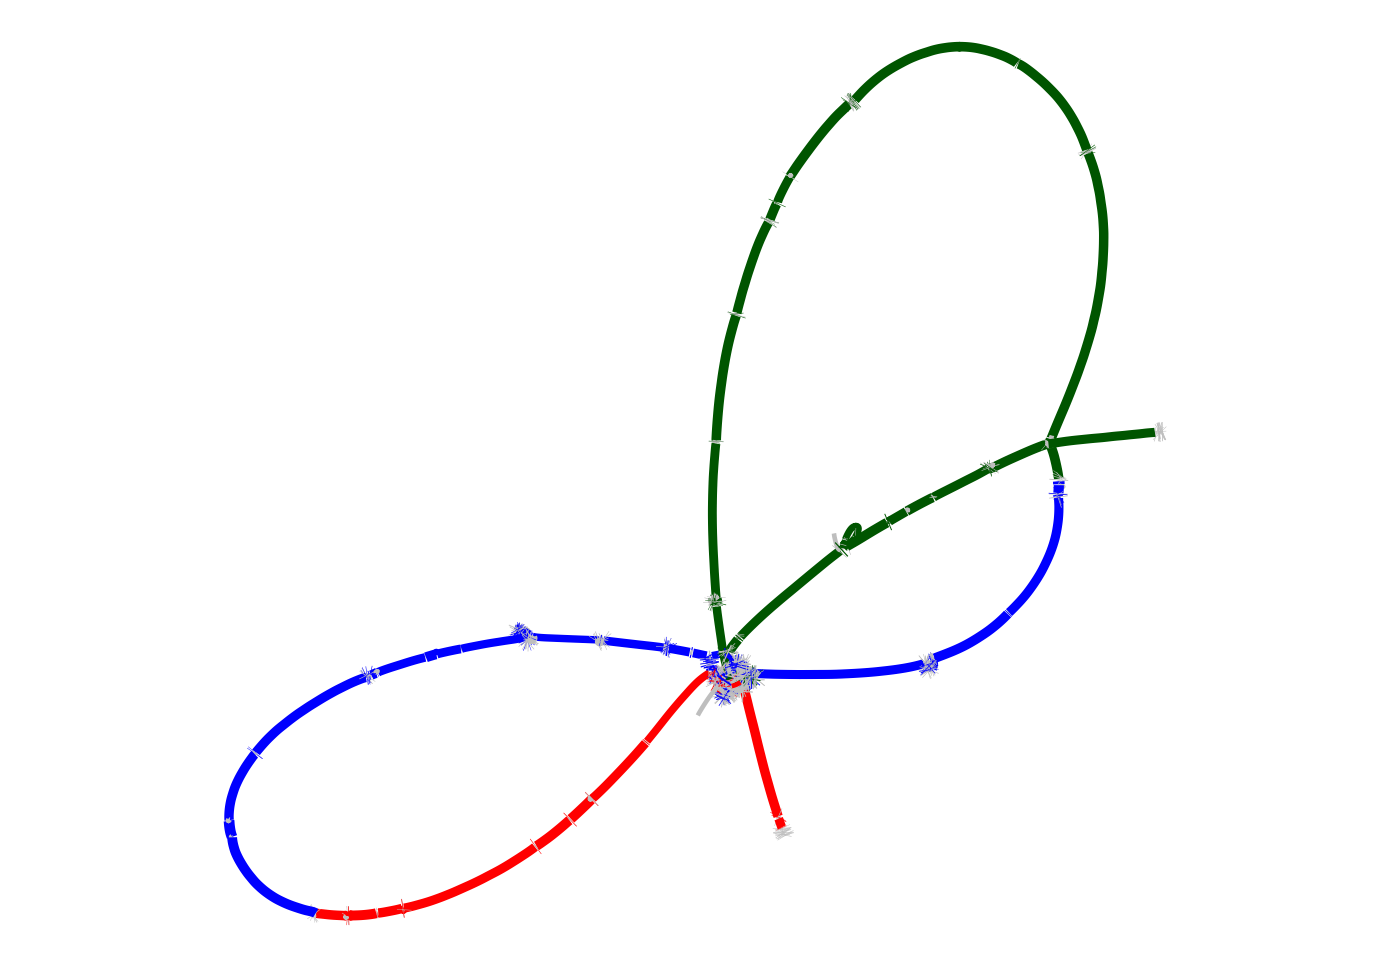
\includegraphics[width=.8\linewidth]{figures/lodelo/tangle_chrCGH_B2_Cgreen_Gblue_Hred.png}
	\caption[Visualization of chromosomes tangle in the \mcactus variation graph.]{ \bandage visualization of the tangle of chromosomes C, G and H in the \mcactus variation graph. Nodes are colored based on \minigraph alignment of chromosome C (dark green), G (blue) and H (red) of the reference assembly B2. The three chromosomes are bound together because of the construction.}
	\label{fig:lodelo_graph_tangle}
\end{figure}

\subsection{Estimating core genome and pangenome growth}
\label{sec:core_pg}
Finally, pangenome graphs are also useful to quantify the part of the genome that is shared between genomes (what is called core-genome) and the parts that are mostly shared or private to each one. It is also interesting to estimate its growth, i.e. to measure how much the total genomic content grows with the increase of the size of the sample. These metrics can be obtained by using the tool \panacus~\cite{panacus}. \texttt{Panacus} is a tool that calculates coverage distributions of countable elements in variation graphs: it uses paths to detect how many genomes are associated to any node, edge or basepair of the pangenome graph. From these distribution it computes the pangenome growth and core curves as function of the number of genomes.\\
Calculating these metrics can be used to validate that the two variation graphs built with \pggb and \mcactus agree on the underlying genetic distribution of the input sample.\\
Figure~\ref{fig:panacus} shows very concordant metrics for the two variation graphs. First, they show similar basepair coverage histogram, that highlight a great portion of genome shared by all the samples, and a non-negligible share of sequences that are private to each genome (~1.5Mbp in total). Secondly, both growth curves show similar pattern, that seems plateauing. This is also highlighted by the fraction of new base pairs introduced by each sample, that decreases from ~700k new basepairs with the new sample to less than ~142k base pairs in on the 11th genome. Finally, the core pangenome can be estimated by the basepairs that are spelled by all the genomes in the graph: the computed value for the 11 samples is ~13,2 Mbp for \pggb and ~13,6 Mbp for \mcactus. The variability in the results are expected and due to different graph construction methods.
\begin{figure}[h!]
	\centering
	\begin{subfigure}[b]{0.45\textwidth}
		\centering
		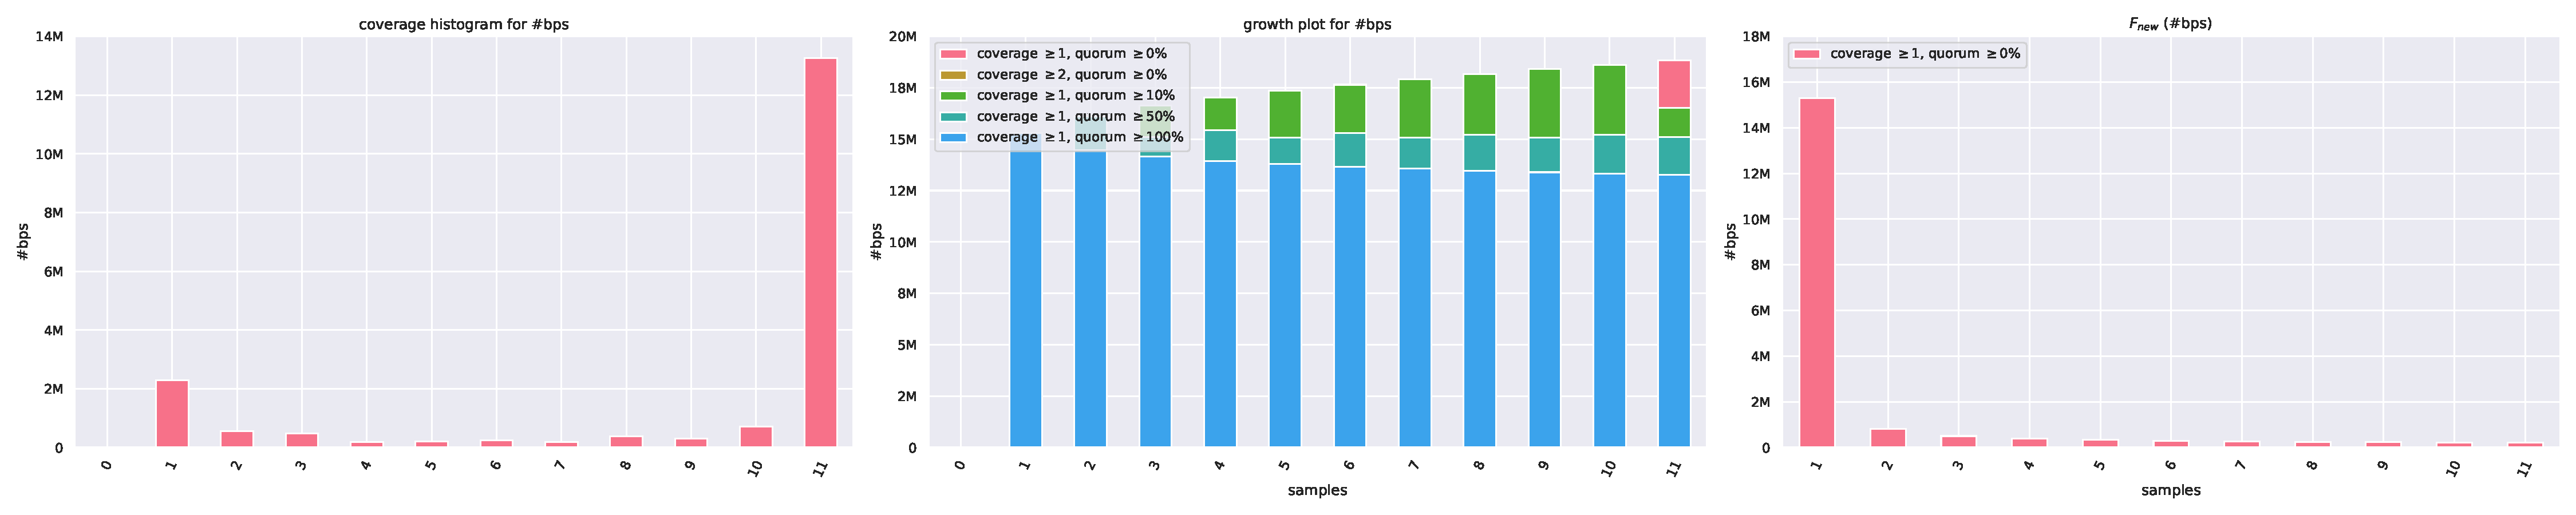
\includegraphics[angle=90,width=.7\textwidth]{figures/lodelo/lodelo_simon.histgrowth.pdf}
		\caption[\pggb pangenome.]{\pggb pangenome.}
	\end{subfigure}%
	\begin{subfigure}[b]{0.45\textwidth}
		\centering
		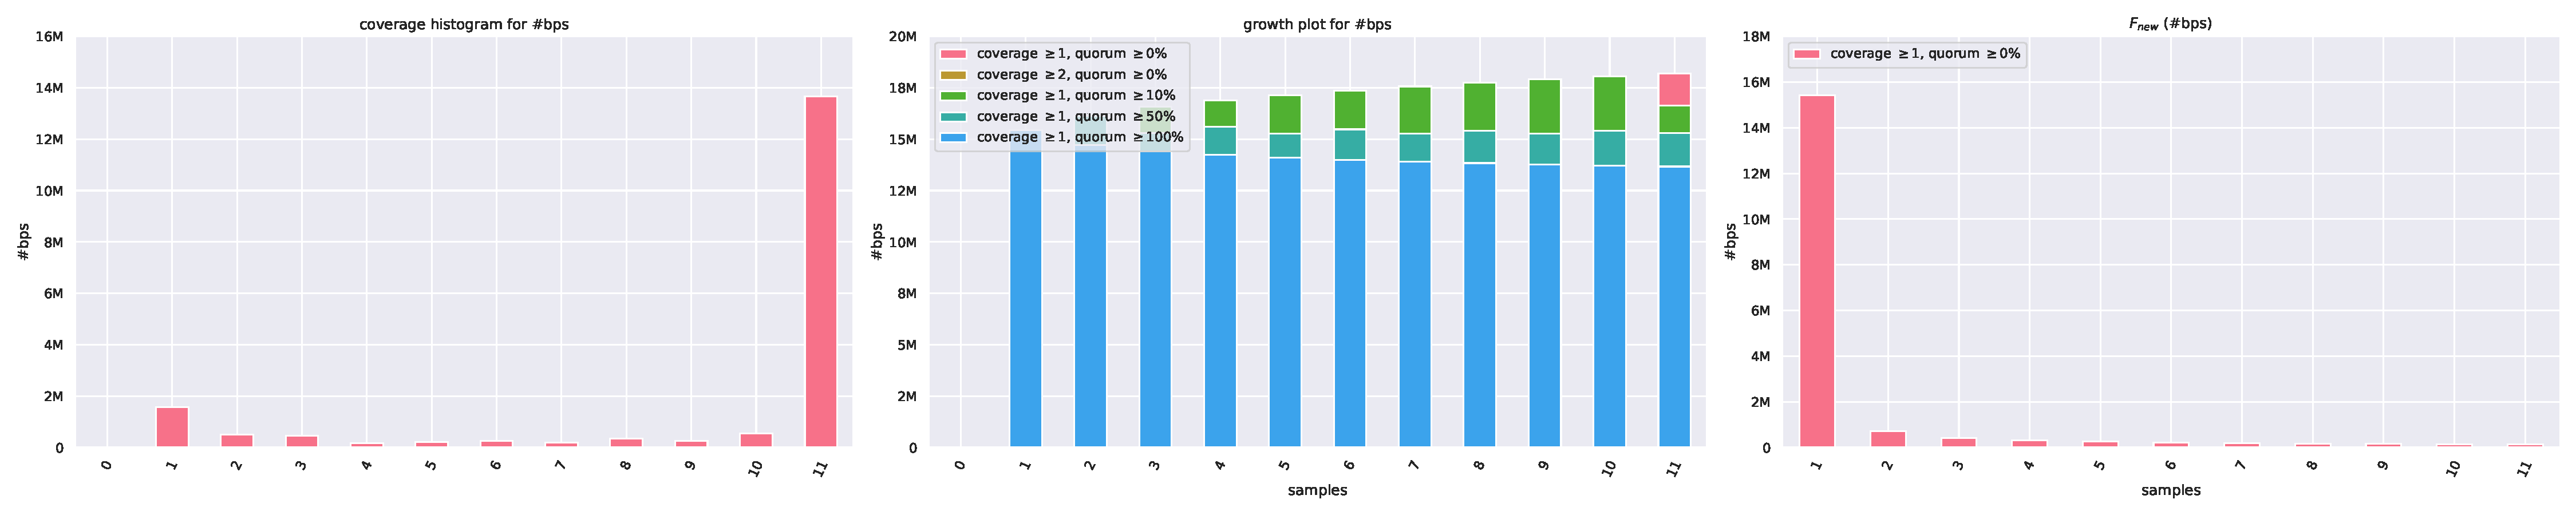
\includegraphics[angle=90,width=.7\textwidth]{figures/lodelo/lodelo_cactus.histgrowth.pdf}
		\caption[\mcactus pangenome.]{\mcactus pangenome.} 
	\end{subfigure}%
	\caption{Pangenome core and growth of \lodelo using variation graphs. \pggb graph generated by Simon Heumos.}
	\label{fig:panacus}
\end{figure}

\section{Conclusion and Perspectives}
The work presented above shows how pangenomes can serve as analysis platform of samples from same-strain yeast. \\
\dbg-based tools currently offer a limited range of possibilities, especially for lower sample sizes. They best serve as fast and memory-efficient container for large amounts of data that require simple interrogations like absence-presence queries. This model can nevertheless help answer simple biological questions on such small samples, like phylogenetic analysis shown in figure~\ref{fig:dbg_phyl}.\\
Variation Graphs on the other side are powerful and very useful on few genomes analysis as they can be built quickly enough and provide a well-established platform for downstream analysis tools. On the other side, there is still need to very labor-intensive manual revision of the output graphs to find the input parameters that produce the best result, as it took more than 25 rounds to find the best \pggb parameters to produce the graph shown in figure~\ref{fig:lodelo_gfaestus}. As they are produced on heuristics and not on mathematically defined concepts, each variation graphs-construction tool produces different results: in figure~\ref{fig:chrE_difference}, it is possible to see the difference 1d-representation of the small chromosome E between \pggb and \mcactus. Finally, in order to detect the inter-chromosomal rearrangement with \mcactus as in figure~\ref{fig:lodelo_graph_tangle}, I had to rewrite the pipeline and modify the input data. \\
Apart from the aforementioned limitations, that show how such methods are still more prototypes than sound and established tools, this analysis shows how much potential there is to improve the current state-of-the art in genomes analysis. Linear-sequences tools are based on well-established genome-to-genome comparison methods that fail to adapt to heterogeneous data, like different levels of assembly quality. As \syri fails to detect rearrangements on genomes that are not assembled to the chromosome level, variation graphs are able to show the variation among all samples, even if the majority of the genomes contain contigs. \\
This work is another display of the great potential pangenome approaches have. In the future it would be very interesting to build pipelines or develop tools that enable visualizations and straightforward analysis from variation graphs or \ccdbgs] to the same level as the current linear-genomes tools. As I have already conceptualized some possible approaches for \ccdbgs, in the future it would be useful to develop simple prototypes and test how fast and precise these would be.\\
In the future it would be very informative to produce a more comprehensive report of the work done by my group and me, together with the other groups that worked on analyzing these novel \lodelo samples, to offer a comprehensive view of how specific pangenomes can be built and used to provide improved genomic analysis capabilities.

\begin{figure}[t]
	\centering
	\begin{subfigure}[b]{0.8\textwidth}
		\centering
		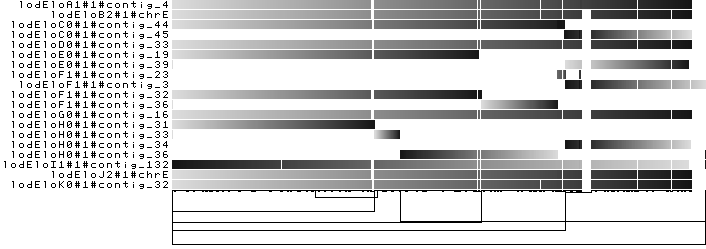
\includegraphics[width=.7\linewidth]{figures/lodelo/chrE.pggb.png}
		\caption{One dimensional visualization of the variation graph built with \pggb, containing 19 contigs from the assemblies, selected before construction using all vs all alignment data.}
		\label{fig:chrE_pggb}
	\end{subfigure}%

	\begin{subfigure}[b]{0.8\textwidth}
		\centering
		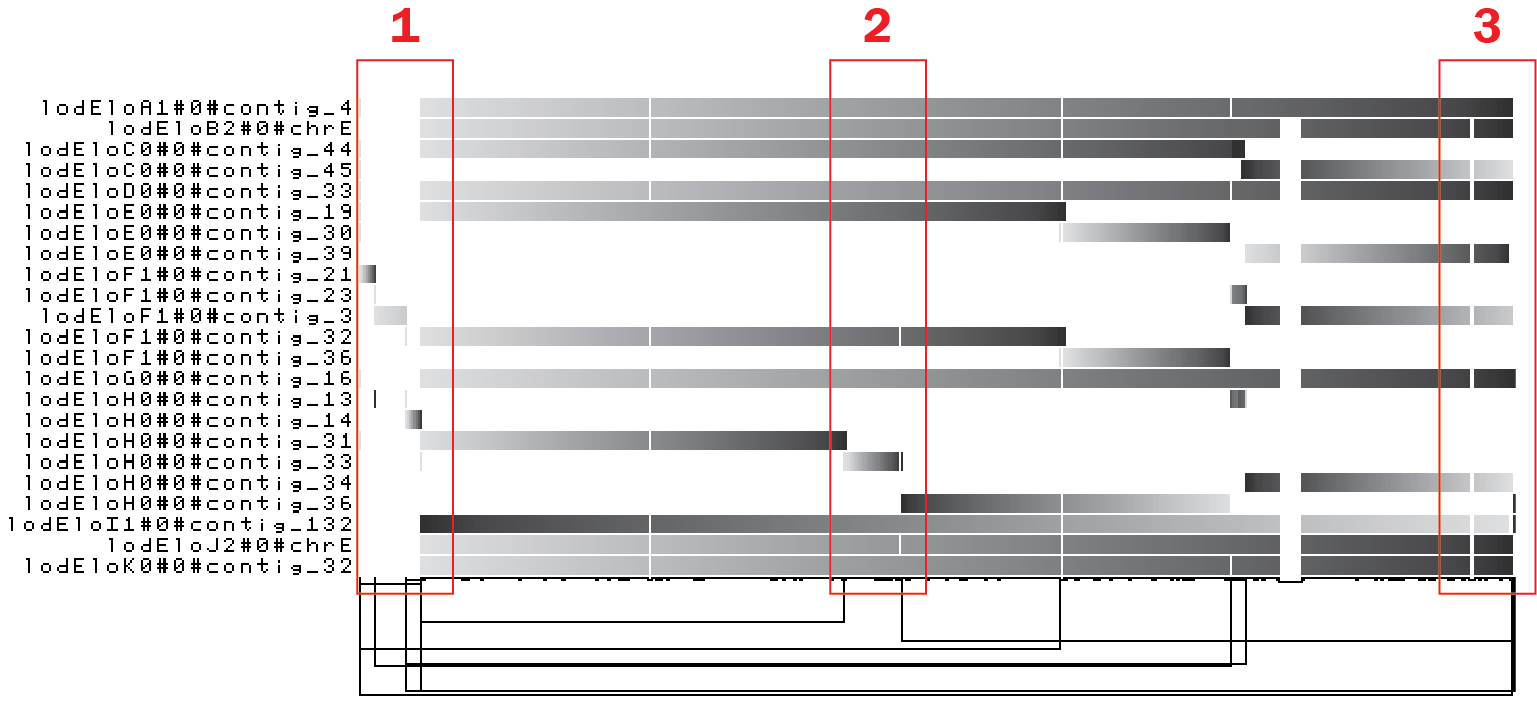
\includegraphics[width=.7\linewidth]{figures/lodelo/chrE.mcactus.png}
		\caption{One dimensional visualization of the variation graph built with \mcactus, containing 23 contigs from the assemblies, selected automatically by the pipeline.}
		\label{fig:chrE_mcactus}
	\end{subfigure}
	\caption[1D visualization of differences between \pggb and \mcactus output.]{One dimensional visualization of chromosome E variation graphs of \pggb and \mcactus using \odgi. Differences can easily be noted in the leftmost parts of the images.}
	\label{fig:chrE_difference}
\end{figure}


\printbibliography